\documentclass[12pt, letterpaper]{report}
\usepackage{fancyhdr}
\usepackage{hyperref}
\usepackage{wrapfig}
\usepackage{subcaption}
\usepackage{graphicx}
\usepackage{multicol}
\usepackage{blindtext}
\usepackage{amsmath}
\usepackage{float}
\usepackage{listings}
\usepackage{xcolor}
\usepackage[margin=1.5cm]{geometry}

\usepackage[english,polish]{babel}
\usepackage[utf8]{inputenc}
\usepackage[T1]{fontenc}
\usepackage{dirtree}
\usepackage{graphicx}
\usepackage{polski}


\graphicspath{ {images/} {images/collisions24x10_2x2} }

\definecolor{codegreen}{rgb}{0,0.6,0}
\definecolor{codegray}{rgb}{0.5,0.5,0.5}
\definecolor{codepurple}{rgb}{0.58,0,0.82}
\definecolor{backcolour}{rgb}{0.95,0.95,0.92}

\lstdefinestyle{codelistingstyle}{
    backgroundcolor=\color{backcolour},   
    commentstyle=\color{codegreen},
    keywordstyle=\color{magenta},
    numberstyle=\tiny\color{codegray},
    stringstyle=\color{codepurple},
    basicstyle=\ttfamily\footnotesize,
    breakatwhitespace=false,         
    breaklines=true,                 
    captionpos=b,                    
    keepspaces=true,                 
    numbers=left,                    
    numbersep=5pt,                  
    showspaces=false,                
    showstringspaces=false,
    showtabs=false,                  
    tabsize=2
}

\lstset{style=codelistingstyle}

\title{
    Praca magisterska \\
    \large Modelowanie elastycznych i nieelastycznych
    zderzeń obiektów\\
    metodą dynamiki molekularnej na potrzeby animacji
    komputerowych
}
\author{
    Kamil Pasterczyk \\
    \small Promotor: dr hab. inż. Tomasz Chwiej
}

\begin{document}

%% ########################################################
\thispagestyle{empty}
\begin{center}
    
\includegraphics[width=0.3\textwidth]{logo_AGH.jpg}\\
    \bf{\sf{WYDZIAŁ FIZYKI I INFORMATYKI STOSOWANEJ}}\\[5mm]
    %% ======================================================
    \bf{\sf{KATEDRA INFORMATYKI STOSOWANEJ I FIZYKI KOMPUTEROWEJ}}\\[14mm]
    \sf{\huge Praca dyplomowa}\\[12mm]
    \sf{\Large Modelowanie elastycznych i nieelastycznych zderzeń obiektów metodą 
    dynamiki molekularnej na potrzeby animacji komputerowych\\[2mm] 
    Molecular dynamics simulations of elastic and inelastic collisions 
    of macroscopic objects in computer animations
    }\\[40mm]
    \end{center}
    \sf{
        \begin{tabular}{ll}
            Autor: & Kamil Pasterczyk\\
            Kierunek studiów: &	Informatyka Stosowana\\
            Opiekun pracy: & dr hab. inż. Tomasz Chwiej, prof. AGH\\
        \end{tabular}
    }\\[10mm]
    \begin{center}
    \sf{Kraków, 2022}
\end{center}

%% ########################################################
\clearpage

\tableofcontents

\chapter{Wprowadzenie}
    \section{Cele projektu}
    Jedną z popularnych metod wykorzystywanych w modelowaniu zderzeń obiektów w mikro- i makroskali jest 
    metoda dynamiki molekularnej. Mimo iż w pierwotnej postaci stosowana była do opisu własności gazów i 
    cieczy, to dzięki swej wszechstronności pozwala modelować obiekty makroskopowe zachowujące kształt 
    przy braku sił zewnętrznych oraz modelować ich rozrywanie w trakcie zderzeń z innymi obiektami.

    Dynamika molekularna to metoda symulacji komputerowej służąca do analizy fizycznych ruchów cząsteczek. 
    Cząsteczki oddziałują ze sobą przez określony czas, dając obraz dynamicznej ewolucji systemu. 
    Trajektorie tych cząsteczek są określane przez numeryczne rozwiązanie równań ruchu Newtona. 
    Ponieważ układy zazwyczaj składają się z bardzo dużej liczby cząstek, niemożliwe jest analityczne 
    określenie właściwości takich złożonych układów. W takich właśnie sytuacjach wykorzystujemy 
    symulacje komputerowe, które co prawda dają wyniki przybliżone, lecz przy dobrym doborze 
    parametrów i dokładności obliczeń możliwe jest odwzorowanie właściwości badanego obiektu. 
    Mimo, iż przeprowadzanie eksperymentów komputerowych obecnie staje się nieodzowne w wielu 
    aspektach działalności naukowej i inżynieryjnej, to należy pamiętać o ich ograniczeniach. 
    Jednym z problemów wykonywania symulacji komputerowych może być ich złe uwarunkowanie, które 
    jest wynikiem kumulowania się błędów numerycznych np. podczas całkowania równań ruchu. 
    Problem ten można starać się zminimalizować poprzez dobór odpowiednich algorytmów lub 
    modyfikację parametrów symulacji. 
    Przykładowo w dowolnym modelu dynamiki molekularnej krytycznym parametrem jest wielkość 
    kroku czasowego. Zbyt duży krok może prowadzić do niestabilności, natomiast zbyt mały 
    prowadzi do wydłużenia czasu wykonywanych symulacji. \\
    
    W pracy został zaadoptowany sparametryzowany model dynamiki molekularnej, który pozwala na 
    symulowanie zderzeń obiektów elastycznych z możliwością ich penetracji i rozrywania. Kluczowym 
    aspektem podczas implementacji algorytmów była wydajność obliczeniowa i dzięki odpowiednim 
    optymalizacjom szybkość wykonywania symulacji pozwala na wizualizację zderzeń w czasie rzeczywistym 
    pod postacią animacji komputerowych. \\

    W projekcie rozważane były jedynie zderzenia obiektów dwuwymiarowych. Pozwala uzyskanie dużo lepszej
    wydajności programu w porównaniu do wersji z trójwymiarowymi obiektami, w której liczba koniecznych obliczeń jest
    znacznie większa. Nie ma jednak istotnych różnic jeżeli chodzi o fizyczny aspekt zderzeń dwu i trzy-wymiarowych, gdyż 
    równania ruchu mają taką samą strukturę a jedynie wartości wektorowe w nich zawarte mają jeden dodatkowy wymiar.


    % --------------------------------------------------------------------------------------------------------------
    \clearpage
    \section{Zastosowane technologie}

    Głównym narzędziem wykorzystamy do stworzenia aplikacji jest \emph{rust}, szybki kompilowany 
    język programowania zapewniający bezpieczeństwo pamięci i łatwe programowanie wielowątkowe. 
    Język ten jest wybierany co roku zaczynając od roku 2015 w ankiecie społeczności \emph{Stack Overflow} jako 
    \emph{``the most beloved programming language''}. O ile jest on wymagający, to jest 
    on również wygodny, kod jest prosty do zrozumienia a programy napisane z jego użyciem 
    można łatwo kompilować na wielu systemach nawet jeżeli używają one zewnętrznych bibliotek, gdyż 
    zależności są zarządzane przez narzędzie \emph{cargo}, będące nieodzowną częścią ekosystemu tego języka.
    Kompilator \emph{rustc} jest restrykcyjny, ponieważ wymusza on na kodzie programu bezpieczeństwo pamięci oraz
    nie zezwala na kod generujący niezdefiniowane zachowanie, będące częstym problemem podczas tworzenia aplikacji
    wielowątkowych. ``Rust breaks down these barriers by eliminating the old pitfalls and providing a friendly, 
    polished set of tools to help you along the way'' - \cite{rustbook}. Surowość kompilatora 
    nie jest poważnym problemem podczas tworzenia aplikacji, ponieważ kompilator dostarcza dokładnego opisu 
    błędu wraz z referencją do dokumentacji a często również sugeruje sposób jego poprawiania. \\

    Na potrzeby zrównoleglenia kodu symulacji wykorzystana została biblioteka \emph{rayon} \cite{rayon}, służąca
    do programowania wielowątkowego w języku \emph{rust} z wykorzystaniem współdzielenia pamięci. 
    Jest to odpowiednik API \emph{OpenMP} ze środowiska wykorzystywanego w 
    programach napisanych w \emph{C} lub \emph{C++}. 
    Do wykonania symulacji na procesorze graficznym wykorzystane zostało API \emph{OpenCL}, jest ono kompatybilne
    z większością obecnie wykorzystywanych systemów operacyjnych i działa ono na sprzętach różnych producentów, 
    w przeciwieństwie do technologii \emph{CUDA}, obsługującej jedynie procesory graficzne \emph{Nvidia}. \\
    
    Do wyświetlania animacji wykorzystane zostało API \emph{\emph{OpenGL}} w profilu rdzennym (core profile), w projekcie
    udostępnione przez bibliotekę \emph{glium}. Nie jest ono już rozwijane, ostatnia stabilna wersja 
    \emph{\emph{OpenGL} 4.6} pojawiła się w roku 2017, jednak jego możliwości są w pełni wystarczające
    na potrzeby projektu. Główne zasady tworzenia programu są takie same jak w nowocześniejszych rozwiązaniach 
    takich jak \emph{Vulkan}, jednak samo API jest nieco łatwiejsze w użyciu i pozwala osiągnąć zamierzone 
    dla tej aplikacji efekty w mniejszej liczbie linijek kodu. \\

    Do wyświetlenia interfejsu graficznego, pozwalającego monitorowanie oraz kontrolowanie stanu symulacji  
    wykorzystana została biblioteka \emph{eGui} \cite{egui}. Jest ona kompatybilna z językiem \emph{Rust} 
    i API \emph{\emph{OpenGL}}, dostarcza możliwości wyświetlania okienek wraz z elementami wejścia (przyciski, suwaki). \\


    % --------------------------------------------------------------------------------------------------------------
    \clearpage
    \section{Wielowątkowość}

    W architekturze komputerowej wielowątkowość to zdolność procesora do 
    jednoczesnego zapewniania wielu wątków wykonywania, obsługiwanych przez 
    system operacyjny. W aplikacji wielowątkowej wątki współdzielą zasoby 
    jednego lub wielu rdzeni, które obejmują jednostki obliczeniowe i pamięci 
    podręczne procesora. Mimo że trudno jest przyspieszyć pojedynczy wątek, 
    większość systemów komputerowych w rzeczywistości wykonuje wiele zadań jednocześnie i 
    w ten sposób są w stanie przyśpieszyć działanie programów. Jeśli wątek nie może wykorzystać 
    wszystkich zasobów obliczeniowych procesora, uruchomienie innego wątku może je wykorzystać i 
    w ten sposób zapobiec marnowania tych zasobów, co jest istotną zaletą programowania wielowątkowego. \\

    Do aplikacji stworzonej na potrzeby pracy dyplomowej zostało wykorzystane podejście 
    tworzenia programów wielowątkowych z współdzieleniem pamięci operacyjnej, 
    czy to pamięci zarządzanej przez CPU (biblioteka \emph{rayon} w języku \emph{Rust}) 
    czy tej zarządzanej przez GPU (API \emph{OpenCL}).
    Bibliotekę \emph{rayon} ma bardzo podobne zastosowanie 
    i sposób działania jak interfejs programowania aplikacji 
    \emph{OpenMP}, powszechnie używany w programach pisanych w językach \emph{C} i \emph{C++}.
    Częstym problemem podczas pisania programów z wykorzystaniem \emph{OpenMP} jest to, że duża 
    dowolność w czytaniu i pisaniu w 
    współdzielonej pamięci operacyjnej może doprowadzić do problemów, takich jak
    zmiana wartości przez jeden wątek podczas gdy inny wątek próbuję ją odczytać, co 
    przy nieprzemyślanej synchronizacji tychże wątków zapewne doprowadzi do niezdefiniowanego
    zachowania się programu.
    Ponieważ język programowania \emph{Rust} bardzo dokładnie kontroluje wszelkie operacje na pamięci 
    współdzielonej, problemy tego typu są bardzo rzadkie podczas pisania wielowątkowego z
    użyciem biblioteki rayon. Odbywa się to kosztem czasu programisty podczas tworzenia 
    oprogramowanie, gdyż musi on zapewnić aby napisany kod spełniał wszystkie restrykcyjne 
    wymagania jak np. "może istnieć tylko jedna mutowalna referencja do danego obiektu". \\

    Jeżeli projektujemy algorytm mający działać na wielu wątkach warto jest pomyśleć o tym, jak
    przedstawić pojedynczy wynik w postaci funkcji zależnej jedynie od danych wejściowych. Jest to 
    możliwe gdy wyniki nie są zależne od siebie i jeżeli proces ten się powiedzie, każdy 
    z wyników może zostać obliczony niezależnie przez jeden wątek.
    ``If you can construct a formula where the output data points can be represented without 
    relation to each other (...) be very happy'' - \cite{cuda}.
    Bardzo pomaga to z problemami synchronizacji,  
    ``Warto rozważyć pisanie kodu wątków w taki sposób, aby każdy wątek działał we 
    własnym świecie, nie współużytkując 
    danych z pozostałymi wątkami.' \cite{cleancode} \\
    
    Gdy tworzymy algorytm mający działać na procesorze graficznym, bardzo istotnym aspektem jest 
    koszt związany z przesyłem danych z pamięci głównej do pamięci karty graficznej. Sam proces kopiowania 
    danych może poważnie wpłynąć na wydajność programu i w niektórych przypadkach może on zająć więcej
    czasu niż samo wykonanie obliczeń.
    ``Computing has (...) moved from one limited by computational throughput of the 
    processor, to one where moving the data is the primary limiting factor'' - \cite{cuda}

    
\chapter{Wstęp teoretyczny}

    Modelowanie zachowania obiektu elastycznego metodą dynamiki molekularnej wymaga określenia 
    położenia jego elementów w przestrzeni. Taki rozkład przestrzenny uzyskuje się opisując 
    obiekt przy pomocy \emph{n} punktów (inaczej nazywanych węzłami), w 
    których skupione są masy. Punkty te oddziałują ze sobą jak w rzeczywistym materiale, ich 
    zbliżanie lub oddalanie się od siebie wymaga przyłożenia sił zewnętrznych.
    ``In the natural sciences one strives to model the complex 
        processes occurring in nature as accurately as possible. 
        The first step in this direction is the description of nature. 
        It serves to develop an appropriate system of concepts.'' - \cite{moleculardynamics}. 
    Ważnym zadaniem modelu jest rzeczywiste odwzorowanie zachowania obiektów elastycznych.

    \begin{equation}
        E_{c} = E_{k} + E_{g} + E_{p} + E_{w} + E_{o}
    \end{equation}

    \begin{equation}
        \frac{d^{2} \vec{r_i}}{dt^{2}} = \frac{\vec{F}}{m_i}
    \end{equation}

    \clearpage
    \section{Siatka węzłów}

    \begin{wrapfigure}{r}{0.50\textwidth}
        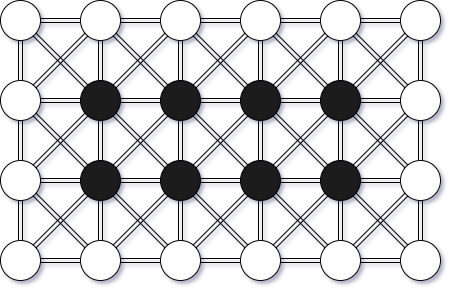
\includegraphics[width=0.95\linewidth]{object_shema.png}
        \caption{
            Siatka węzłów reprezentująca obiekt kwadratowy - 
            czarnym kolorem oznaczone zostały węzły wewnętrzne a białym węzły zewnętrzne.
        }
    \end{wrapfigure}

    Rzeczywiste obiekty znane z realnego świata są trójwymiarowe. Jednak zdarza się, że rozmiary przestrzenne 
    obiektu w jednym z trzech kierunków są znacznie mniejsze od dwóch pozostałych. Wówczas taki obiekt można 
    opisywać stosując przybliżenie dwuwymiarowe, gdyż efekty dynamiczne związane z tymi dwoma kierunkami 
    stają się dominujące względem trzeciego (np. zmiana długości pod wpływem sił zewnętrznych). 
    W metodzie dynamiki molekularnej modele dwu i trzy wymiarowe koncepcyjnie niczym się nie różnią, 
    jednak redukcja wymiarowości pozwala zwiększyć wydajność obliczeniową. 
    Taki był też powód zastosowania przybliżenia 2D w tej pracy.

    W naszym modelu obiekt elastyczny reprezentowany jest przez dwuwymiarową 
    siatkę węzłów. Węzły oddziałują ze swoimi sąsiadami siłami typu 
    Lennarda-Jonesa lub harmonicznymi opisanymi w dalszej części pracy.


    Przy tych założeniach oddziaływanie dla węzłów w środku będzie izotropowe (niezależne od kierunku). 
    Węzły brzegowe mają mniej sąsiadów i w pewnych warunkach mogą zachowywać się inaczej niż węzły w środku, 
    ich wychylenia z położenia równowagi będą większe podczas zderzeń ze ścianką. Są one z tych powodów 
    bardziej podatne na oderwanie się od reszty siatki. Zbyt duża siła przyłożona do węzłów brzegowych 
    może również spowodować nieodwracalną deformację siatki, jest to bardziej prawdopodobne podczas 
    używania większych kroków czasowych.
    
    \subsection{Liczba najbliższych sąsiadów}
    Oddziaływania międzycząsteczkowe liczone są tylko pomiędzy kilkoma lub kilkunastoma najbliższymi 
    sąsiadami, w celu zmniejszenia ilości wymaganych obliczeń. W pracy oddziaływanie między węzłami 
    modelowane jest przy użyciu krótkozasięgowego potencjału Lennarda-Jonesa, który na dużych 
    odległościach szybko zbliża się do zera. Liczenie oddziaływań pomiędzy bardzo oddalonymi od 
    siebie cząsteczkami nie wpływa znacząco na wynik, wymaga jednak znacznego nakładu obliczeniowego, 
    czego zazwyczaj unika się podczas wykonywania symulacji numerycznych.


    \clearpage
    \section{Model oddziaływań}

    \begin{wrapfigure}{l}{0.30\textwidth}
        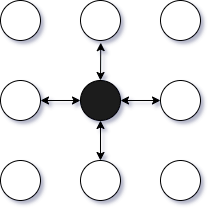
\includegraphics[width=0.95\linewidth]{four_nebiours.drawio.png} 
        \caption{Połączenie obiektów używając sąsiedztwa von Neumanna}
        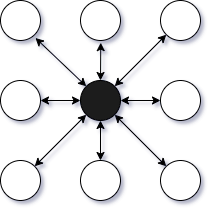
\includegraphics[width=0.95\linewidth]{eight_nebiours.drawio.png} 
        \caption{Połączenie obiektów używając sąsiedztwa Moore\'a}
    \end{wrapfigure}

    Potencjał Lennarda-Jonesa został wykorzystany do symulacji przyciągania/odpychania 
    węzłów w jednym obiekcie, symulacji kolizji węzłów ze ścianami oraz symulacji
    kolizji węzłów z węzłami należącymi do innych obiektów. 
    Potencjał ten opisany jest za pomocą poniższego równania:
    \begin{equation}
        E_{LJ} = V_0 \left[ \left( \frac{\sigma}{l} \right)^{12} - \left( \frac{\sigma}{l} \right)^{6} \right]
    \end{equation}
    \begin{equation}
        \sigma = \frac{d_0}{\sqrt[6]{2}}
    \end{equation}
    Gdzie $l$ to odległość między dwiema oddziałującymi cząstkami, $V_0$ to współczynnik określający wielkość potencjału 
    a $\sigma$ to odległość, przy której energia potencjalna oddziaływania pomiędzy cząsteczkami wynosi zero. 
    Potencjał Lennarda-Jonesa ma swoje minimum w odległości $d_0 = \sqrt[6]{2} \sigma$. \\ \\
    Siła zdefiniowana jest jako pochodna energii:
    \begin{equation}
        F_{LJ} = 
        \frac{d}{dl} E_{LJ} = 
        \frac{d}{dl} V_0 \left[ \left( \frac{\sigma}{l} \right)^{12} - \left( \frac{\sigma}{l} \right)^{6} \right]
    \end{equation}
    \begin{align*}
        F_{LJ} &= \frac{d}{dl} V_0 \left[ \sigma^{12}l^{-12} - \sigma^{6}l^{-6} \right] =\\
        &= V_0 \left[ 6\sigma^{6}l^{-7} - 12\sigma^{12}l^{-13} \right] =\\
        &= 3 V_0 \left[ (d_{0})^{6} l^{-7} - (d_{0})^{12} l^{-13} \right] =\\
        &= 3\frac{V_0}{d_0} \left[ \left(\frac{d_0}{l}\right)^{7} - \left(\frac{d_0}{l}\right)^{13} \right]
    \end{align*}
    W ten sposób otrzymaliśmy wzór opisujący siłę wynikającą z potencjału Lennarda-Jonesa:
    \begin{equation}
        F_{LJ} = 3\frac{V_0}{d_0} \left[ \left(\frac{d_0}{l}\right)^{7} - \left(\frac{d_0}{l}\right)^{13} \right]
    \end{equation}

    \clearpage
    % --------------------------------------------------------------------------------------------------------------
    \section{Wielkości fizyczne wyznaczane używając metodę dynamiki molekularnej}
    Korzystając z modelu można wyznaczyć i zaprezentować wartości fizyczne opisujące układ jak 
    na przykład temperatura czy ciśnienie. Mając do dyspozycji takie metody obliczeniowe jak dynamika 
    molekularna, możemy oprócz wizualizacji zderzeń obiektów, analizować również takie wielkości fizyczne rozkład
    temperatury lub ciśnieni wewnątrz obiektów. Taka analiza jest istotna w przypadku generowania
    realistycznych symulacji jak na przykład rozrywanie elastycznego materiału czy 
    zderzenie meteorytu z powierzchnią planety. Takie dodatkowe informacje potrafią ukazać skalę 
    zawartej w układzie energii.

    \subsection{Temperatura z zasady ekwipartycji energii}
    Punktem wyjścia może być zasada ekwipartycji energii: średnia energia kinetyczna na jeden stopień swobody jest równa 
    $\frac{k_{B}T}{2}$ gdzie $k_{B}$ to stała Boltzmanna a $T$ to temperatura.

    \begin{equation}
        \left< E_{k} \right> = s \frac{k_{B}T}{2}
    \end{equation}

    W naszym przypadku liczba stopni swobody $s = 2$ (ruch translacyjny w dwóch kierunkach $x$ i $y$).

    \begin{align*}
        \left< E_{k} \right> = \left< \frac{m v^{2}}{2} \right> = \frac{m}{2} \left< v^{2} \right> = T \frac{k_{B}}{2}
    \end{align*}

    \begin{equation}
        T = \frac{m}{k_{B}} \left< v^{2} \right>
    \end{equation}

    Jest to najprostsze przybliżenie temperatury, dotyczące gazu doskonałego, w którym cząstki gazu 
    wzajemnie ze sobą nie oddziałują. Wzór ten wymaga modyfikacji w celu uzyskania właściwego wyniku. \\

    Rozważmy przypadek gdy obiekt porusza się w przestrzeni jako całość: swobodny spadek w polu grawitacyjnym.
    Węzły nie drgają i przemieszczają się z tą samą prędkością:
    $\vec{V_k} = \vec{V_0} + \vec{g}t$ dla $t > 0  \Rightarrow  |\vec{V_k}|^2  \Rightarrow  T > 0$ a 
    przecież swobodny spadek nie rozgrzewa ciał. 
    Możemy zatem wnioskować, że powyższy wzór jest nieodpowiedni dla naszego modelu, 
    należy go zmodyfikować wprowadzając odpowiednie poprawki.
    
    \subsection{Modyfikacja wzoru}
    Pierwszym wykonanym krokiem w celu poprawy wzoru jest przeskalowanie prędkości, co oznacza odjęcie 
    średniej prędkość z jaką porusza się obiekt jako całość, wówczas nie będzie
    to prowadziło dodatkowego wzrostu temperatury. 
    \begin{equation}
        \left< v^{2} \right> = \frac{1}{T} \int_{0}^{T} v^2(t) dt
    \end{equation}
    Estymator $\left< v^{2} \right>$ to średnia arytmetyczna: 
    $t = t_i = i \cdot \Delta t$ dla $i = 0, 1, ..., n-1$. Przy czym \emph{n} musi być na tyle małe
    abyśmy uśredniali jedynie po krótkim odcinku czasu.

    \begin{equation}
        \left< v^{2} \right>  \approx  \overline{v^2} = \frac{1}{n \cdot \Delta t} \sum_{i = 0}^{n} {v_i}^2 \Delta t
        = \frac{1}{n} \sum_{i = 0}^n {v_i}^2
    \end{equation}

    Modyfikujemy wzór odejmując wartość średnią (wariancję):
    \begin{align*}
        \left< \left( v - \left< v \right> \right)^2 \right>  &=  
        \frac{1}{T} \int_{0}^{T} \left( v(t) - \left< v \right> \right)^2 dt  \\
        &= \frac{1}{T} \int_{0}^{T} \left( v^2(t) - 2v \left< v \right> + \left< v \right>^2 \right) dt  \\
        &= \frac{1}{T} \int_{0}^{T} v^2 \, dt - 2 \left< v \right> \frac{1}{T} \int_{0}^{T} v \, dt + \left< v \right>^2 
        + \left< v \right>^2 \frac{1}{T} \int_{0}^{T} dt \\
        &= \left< v^2 \right> - 2 \left< v \right> \cdot \left< v \right> + \left< v \right>^2 \\
        &= \left< v^2 \right> - \left< v \right>^2
    \end{align*}

    Uzyskany wynik to wariancja prędkości:
    \begin{equation}
        {\delta_v}^2  =  \left< \left( v - \left< v \right> \right)^2 \right>  =  \left< v^2 \right> - \left< v \right>^2
    \end{equation}

    Estymator wariancji:
    \begin{equation}
        {\delta_v}^2  \approx  \frac{1}{n} \sum_{i = 0}^{n - 1} {v_i}^2 - \left( \frac{1}{n} \sum_{i = 0}^{n - 1} {v_i} \right)^2
    \end{equation}

    Powyższy wzór zawiera już poprawkę eliminując z niego ruchu postępowego środka masy układu.
    Ponownie rozparzymy spadek swobodny dla jednego wymiaru: $v_k = v_0 + gt$ gdzie $v_0 = 0 = v_k = gt$

    \begin{align*}
        {\delta_v}^2  &=
        \left< v^2 \right> - \left< v \right>^2 \\ 
        &=  \frac{1}{T} \int_{0}^{T} g^2 t^2 \, dt  -  \left( \frac{1}{T} \int_{0}^{T} g \cdot t \, dt \right)^2  \\
        &=  g^2 \frac{1}{T} \frac{T^3}{3}  -  \left( g \frac{1}{T} \frac{T^2}{2} \right)^2  = \frac{g^2 T^2}{3}  -  \frac{g^2 T^2}{4} \\
        &=  \frac{g^2 T^2}{12}
    \end{align*}

    \begin{equation}
        {\delta_v}^2  =  \frac{g^2 T^2}{12}
    \end{equation}

    Z powyższych obliczeń wynika, że temperatura wciąż wzrasta podczas swobodnego spadku
    ale jednak wzrost ten jest mniejszy o jeden rząd wielkości. 
    Jeżeli jednak $a >> g$ to wpływ na temperaturę jest niewielki a dla $T << 1$ oraz $a >> g$ 
    na przykład dla $a = 5 \cdot g \Rightarrow {\delta_{v_a}}^2 = 25 \cdot {\delta_{v_g}}^2$.
    Zastosowanie powyższej metody do wyznaczania temperatury jest problematyczne nawet po wprowadzeniu do niej poprawek i
    ze względu na powyżej przedstawione problemy oraz trudną implementację nie została ona 
    wykorzystana w dalszej części pracy. 

    \clearpage
    % --------------------------------------------------------------------------------------------------------------
    \section{Temperatura z twierdzenia o wiriale}
    Kolejnym podejściem było uzyskanie energii potencjalnej i kinetycznej z twierdzeniu o wiriale.
    Prędkości węzłów zmieniają się w czasie, więc będzie też zmieniać się średnia energia kinetyczna układu
    a przez to i rozkład temperatury.

    \begin{equation}
        \left< E_{kinetyczna} \right>  =  \left< \sum_{k = 1}^{N_p} \frac{m_k}{2} {v_k}^2 \right>
        = \sum_{k = 1}^{N_p} \frac{m_k}{2} \left< {v_k}^2 \right>
    \end{equation}

    Twierdzenie o wiriale mówi że energia kinetyczna zmienia się wskutek oddziaływań wewnętrznych i można ją 
    liczyć ze wzoru:

    \begin{equation}
        \left< E_{kinetyczna} \right>  = 
         - \frac{1}{2} \sum_{k = 1}^{N_p} \left< \vec{F_k} \cdot \vec{r_k} \right>
    \end{equation}

    \begin{equation}
        \vec{F_k} = \sum_{j = 1}^{M} \vec{{F_k}_j}
    \end{equation}
    Gdzie $N_p$ to liczba węzłów w układzie, $M$ to liczba sąsiadów a $\vec{{F_k}_j}$ to siła oddziaływania z sąsiadem $j$-tym.

    \begin{equation}
        \left< E_{kinetyczna} \right> = 
        \sum_{k = 1}^{N_p} -\frac{1}{2} \left< \vec{F_k} \cdot \vec{r_k} \right>_t =
        \sum_{k = 1}^{N_p} \left< E_{kinetyczna} , k \right>_t
    \end{equation}
    $\left< E_{kinetyczna} , k \right>$ to suma średnich energii kinetycznych węzłów. Dla każdego węzła $k$ możemy policzyć:

    \begin{equation}
        \left< E_{kinetyczna} , k \right> = 
        -\frac{1}{2} \frac{1}{\tau} \int_{0}^{\tau} \vec{F_k}(t) \cdot \vec{r_k}(t) \, dt
    \end{equation}
    Gdzie $\tau = \Delta t \cdot n$.

    \begin{equation}
        \left< E_{kinetyczna} , k \right> = 
        -\frac{1}{2} \frac{1}{n} \sum_{j = 0}^{n} \left[  F_{kx}(t_j) \cdot x_n(t_j) + F_{ky}(t_j) \cdot y_k(t_j) \right]
    \end{equation}
    Elementy sumy zapisywane są tak samo jak poprzednio w tablicy. Przyjmujemy $n > 100$ lub więcej. 

    \begin{equation}
        \left< E_{kinetyczna, k} \right> = k_B T_k \Rightarrow T_k = \frac{\left< E_{kinetyczna, k} \right>}{k_B}
    \end{equation}
    Gdzie $k_B$ to stała Boltzmanna a $T_k$ to obliczona temperatura. \\

    Warto zwrócić uwagę na właściwości powyższego wzoru:
    \begin{enumerate}
        \item Jeśli $\vec{F_n} = 0 \Rightarrow T_k = 0$ czyli temperatura jest taka jak temperatura otoczenia.
        \item Jeśli $\left< E_{kinetyczna, k} \right> < 0 \Rightarrow T_k < 0$ oznacza że lokalna 
        temperatura stało się mniejsze niż w otoczeniu obiektu.
    \end{enumerate}

    \clearpage
    % --------------------------------------------------------------------------------------------------------------
    \subsection{Obliczanie temperatury}
    \begin{wrapfigure}{R}{0.35\textwidth}
        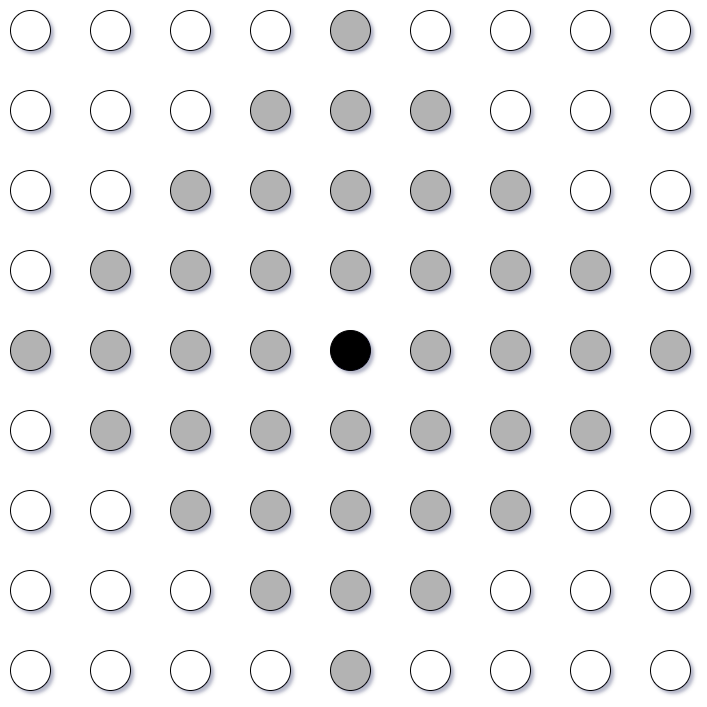
\includegraphics[width=0.95\linewidth]{avg.drawio}
        \caption{
            Obliczanie uśrednionej w przestrzeni temperatury.
            Temperatura obliczana jest dla węzła o kolorze czarnym, 
            natomiast węzły szare są jego sąsiadami.
        }
    \end{wrapfigure}

    Obliczona za pomocą powyższych wzorów temperatura wykazywała się bardzo dużą zmiennością w czasie,
    powodując bardzo szybką zmianę kolorów węzłów, co poważnie utrudniało analizę stanu symulacji. 
    Z tego powodu ostateczny kolor węzła w widoku temperatury kalkulowany jest w następujący sposób:
    \begin{enumerate}
        \item Dla każdego węzła obliczamy temperaturę wedle wzoru i zapisujemy ją wraz z czasem w
        symulacji do tablicy, każdy węzeł ma osobną tablicę.
        \item Dla każdego węzła $n$ obliczamy średnią temperaturę w czasie, w ten sposób każdemu węzłowi
        odpowiada jedna liczba.
        \item Ostateczna temperatura jaka będzie wyświetlona w widoku temperatury dla węzła $n$
        jest sumą uśrednionych w czasie temperatur z czterech rzędów węzłów sąsiadujących z
        węzłem $n$.
    \end{enumerate}

    % Dla każdej cząsteczki tworzymy rejestr w postaci tablicy. 
    % Suma średnich energii $E_{kinetyczna}$ obliczana jest w każdej chwili czasowej.
    % Aby ustabilizować rezultaty, energia kinetyczna dla węzła będzie obliczana jako 
    % średnia z $n$ ostatnich chwili czasowych a ostateczna temperatura jest uśredniana dla 
    % Do rejestru dostajemy się za pomocą dzielenia modulo $j = i \, \%  \, n$, które gwarantuje, 
    % że nie wyjdziemy poza tablicę oraz stare wartości będą nadpisywana na bieżąco. \\

    Obliczanie temperatury przy użyciu twierdzenia o wiriale okazało się być bardziej intuicyjne i
    wyraźnie łatwiejsza w implementacji, dlatego ta metoda została użyta w aplikacji do stworzenia widoku 
    temperatury węzłów, przedstawionego w dalszej części pracy.
    
    % --------------------------------------------------------------------------------------------------------------
    \section{Obliczanie ciśnienia na węźle}
    Lokalne zmiany temperatury informują nas o dynamice zachodzących zmian w obiekcie.
    Inne wielkości, które mogą dostarczać nam informacji o stanie układu jest ciśnienie.
    W stanie o dużej dynamice, rozkład temperatury i ciśnienia są ze sobą połączone, gdyż 
    pokazują rozchodzenie się energii zderzenia w obiekcie. Różnica ujawnia się w przypadku statycznym,
    gdy $T_k = 0$, i węzły nie przemieszczać się względem siebie ale wywierają na siebie duży wpływ poprzez 
    ciśnienie, dające obraz ilości zakumulowanej w obiekcie energii.

    W celu obliczenia ciśnienia działającego na węzeł, zamykamy go w komórce 
    o boku $\Delta = 2 dx$. Wybór $dx$ pozostawia pewną dowolność jednak powinno być ono małe, najlepiej aby było wyraźnie 
    mniejsze niż najmniejsza odległość równowagi pomiędzy dwoma połączonymi węzłami, na przykład $d_0 > 10 dx$. 
    Obliczamy pochodną siły jaka oddziaływała 
    by na węzeł gdyby został on przemieszczony o $dx$ w każdym z czterech kierunków. 
    Będziemy w tym celu potrzebować pochodnej z siły Lennarda-Jonesa:
    \begin{equation}
        F_{LJ} = 
        \frac{d}{dl} E_{LJ} = 
        \frac{d}{dl} V_0 \left[ \left( \frac{\sigma}{l} \right)^{12} - \left( \frac{\sigma}{l} \right)^{6} \right]
    \end{equation}
    \begin{equation}
        \frac{d}{dl} F_{LJ} = 3\frac{V_0}{(d_0)^2} \left[ -7 \left(\frac{d_0}{l}\right)^{8} + 13 \left(\frac{d_0}{l}\right)^{14} \right]
    \end{equation}
    
    \clearpage
    Wykorzystując powyżej obliczoną pochodną jesteśmy teraz z stanie opisać ciśnienie 
    na ściankach w dwuwymiarowym układzie za pomocą wzoru:
    \begin{equation}
        P_x (x \pm \frac{\Delta}{2}) = \frac{F_x (x \pm \frac{\Delta}{2})}{\Delta}
    \end{equation}
    \begin{equation}
        F_x (x + \frac{\Delta}{2}) = F_x (x) + \frac{\partial F_x}{\partial x} 
        \left| _{x + \frac{x}{2}}  \frac{x}{2} + \frac{\partial^2 F_x}{\partial x^2 }  \right| \frac{\Delta^2}{4} + O(\Delta^3)
    \end{equation}
    \begin{equation}
        F_x (x - \frac{\Delta}{2}) = F_x (x) - \frac{\partial F_x}{\partial x} 
        \left| _{x - \frac{x}{2}}  \frac{x}{2} + \frac{\partial^2 F_x}{\partial x^2 }  \right| \frac{\Delta^2}{4} + O(\Delta^3)
    \end{equation} 
    \begin{equation}
        \Delta F_x = 
        F_x (x - \frac{\Delta}{2}) - F_x (x - \frac{\Delta}{2}) = 
        \frac{\Delta}{2} \left[ \frac{\Delta F_x}{\partial x} |_{x + \frac{\Delta}{2}}  -
          \frac{\Delta F_x}{\partial x}|_{x - \frac{\Delta}{2}} \right] + O(\Delta^2)
    \end{equation}

    \begin{wrapfigure}{l}{0.45\textwidth}
        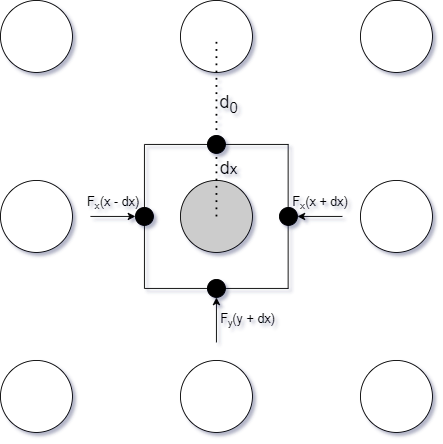
\includegraphics[width=0.9\linewidth]{pressure_box}
        \caption{Schemat komórki przeznaczonej do obliczania ciśnienia na węźle}
    \end{wrapfigure}

    Dzielimy równanie przez $\Delta$:
    \begin{equation}
        p_x = \frac{\Delta F_x}{\Delta} = \frac{1}{2} 
        \left[ \frac{\partial F_x}{\partial x} |_{x + \frac{\Delta}{2}} - \frac{\partial F_x}{\partial x} |_{x - \frac{\Delta}{2}} \right] + O(\Delta)
    \end{equation}

    Podobnie liczymy dla kierunku $y$:
    \begin{equation}
        p_y = \frac{\Delta F_y}{\Delta} = \frac{1}{2} 
        \left[ \frac{\partial F_y}{\partial y} |_{y + \frac{\Delta}{2}} - \frac{\partial F_y}{\partial y} |_{y - \frac{\Delta}{2}} \right] + O(\Delta)
    \end{equation}

    A następnie uśredniamy:
    \begin{equation}
        p_{srednie} = \frac{1}{2} \left( -p_x - p_y \right)
    \end{equation}
    Dodajemy ujemny znak do $p_x$ oraz $d_x$ ponieważ siła jest skierowana do środka komórki a 
    ciśnienie powinno być większe od zera. Dla każdego węzła należy policzyć pochodne siły w czterech punktach w celu 
    uzyskania wartości działającego na niego ciśnienia. Warto zwrócić uwagę na eliminację wpływu 
    pola grawitacyjnego na obliczone ciśnienie, ponieważ jest to wartość stała, której wkład znika po zróżnicowaniu.

    \clearpage
    % --------------------------------------------------------------------------------------------------------------
    \section{Algorytm Verleta}
    Dysponując modelem matematycznym układu,
    możemy ge opisać pod warunkiem że jesteśmy w stanie rozwiązać układ 2N równań różniczkowych 
    drugiego rzędu jakie jakie otrzymujemy z równań ruchu dla całego układu złożonego z N węzłów siatki.
    W ogólnym przypadku, rozwiązanie analityczne nie jest możliwe i jedynym sposobem jego rozwiązania 
    jest użycie metod numerycznych a dokładniej jednej z metod dedykowanych dla problemów jednostkowych.
    Spośród dostępnych metody jak np. metody Eulera, metody RK4, metody wielokrokowej (Adams-Baskjert, Adams-Moulibu)
    lub wybrany na cele projektu metoda Verleta.

    Rząd dokładności schematu verleta. Porównanie wersję prędkościową i położeniową algorytmu Verleta.
    Schemat prędkościowy jest użyteczny ponieważ w niektórych tłumienie i tarcie w modelu zależą od prędkości. \\


    Do całkowania przyśpieszenia wybrany został algorytm prędkościowy \emph{Verleta}. 
    Jest to metoda numeryczna stosowana do całkowania równań ruchu Newtona,
    jest często używana do obliczania trajektorii cząstek w symulacjach 
    dynamiki molekularnej i grafice komputerowej.
     
    ``The velocity form of the Verlet algorithm is one in
        which $v_{n}$ appears directly in the equations to be iterated.
        These equations retain the superior numerical precision
        of the summed form.'' - \cite{velocityverlet}.
    Kroki jakie należy wykonać w celu wykorzystania algorytmu Verleta na 
    potrzeby symulacji fizycznej prezentują się następująco:
    \begin{enumerate}
        \item Obliczamy nowe pozycje pozycję dla każdego węzła: 
        $\vec{x}(t + \Delta t) = \vec{x}(t) + \vec{v}(t) \Delta t + \frac{1}{2} \vec{a}(t) (\Delta t)^2$

        \item Korzystając z nowych pozycji $\vec{x}(t + \Delta t)$ obliczamy nowe 
        przyśpieszenie $\vec{a}(t + \Delta t)$ jednocześnie 
        zachowując $\vec{a}(t)$ - jego poprzednią wartość.

        \item Wykorzystując uzyskane w poprzednich krokach wartości wyznaczamy nową prędkość dla każdego z węzłów 
        $\vec{v}(t + \Delta t) = \vec{v}(t) + \frac{1}{2} \left( \vec{a}(t) + \vec{a}(t + \Delta t) \right) \Delta t$
    \end{enumerate}

    ``Jego podstawową zaleta jest większa dokładność przy 
    niewiele większym (od algorytmu Eulera) koszcie obliczeniowym. 
    Jest przy tym łatwy w implementacji, dokładny i stabilny.'' - \cite{numerical}.

    Integracja Verleta zapewnia dobrą stabilność numeryczną a także posiada inne właściwości, które 
    są ważne w układach fizycznych, jak na przykład odwracalność w czasie. Możliwości tej metody nie są 
    okupione znaczącymi dodatkowymi kosztami obliczeniowymi w porównaniu z prostą metodą \emph{Eulera}. 
    Inne metody takie jak algorytm \emph{RK4} cechują się lepszą dokładnością ale za 
    to wymagany nakład obliczeniowy jest znacznie większy, co mogło by negatywnie wpłynąć na płynność animacji,
    i z tego powodu nie został on zastosowany podczas tworzenia aplikacji.

\chapter{Implementacja}

    \section{Struktura projektu}
    Projekt posiada dwa pliki wykonywalne, jeden służy jako pomoc do generowania scen, które zapisywane są 
    do plików. Drugi plik jest wykonywalny po podaniu ścieżki do pliku zawierającego scenę wyświetla ją, 
    udostępnia interfejs i pozwala na wykonywanie i monitorowanie symulacji. Struktura repozytorium
    prezentuje się następująco: \\

    \dirtree{%
        .1 elastic-objects-rs.
        .2 data.
        .2 doc.
        .3 code.
        .3 images.
        .2 glsl.
        .2 scenes.
        .2 src.
        .3 bin.
        .3 kernels.
        .3 scene.
        .3 simulation.
    }

    \begin{enumerate}
        \item Folder \emph{src} zawiera główny kod źródłowy programu.
        
        \item Znajduje się w nim folder \emph{bin} zawierający pliki wykonywalne, 
        jeden służący do generowania scen, drugi do wykonywania symulacji. 

        \item Wygenerowane stany symulacji domyślnie zapisywane i czytane są z folderu \emph{scenes}.
        
        \item W folderze \emph{kernels} znajduje się kod wykorzystywany przez \emph{OpenCL} do 
        wykonywania symulacji na procesorze graficznym.
        
        \item Pliki generowane przez symulację zapisywane są w folderze \emph{data}. 
        Są to logi zawierające informacje o stanie energii symulacji w danych chwilach czasowych.

        \item W folderze \emph{glsl} znajdują się kod shaderów wykorzystywanych do rysowania stanu symulacji.
    \end{enumerate}

    \clearpage
    % --------------------------------------------------------------------------------------------------------------
    \section{Węzły}
    Informacje o węzłach znajdujących się w symulacji są przechowywane w strukturze \emph{Node}.

    \lstinputlisting[language=C]{code/node.rs}
    Atrybut $repr(C)$ zapewnia taką samą reprezentację obiektu w pamięci jak, gdyby była to
    struktura w języku \emph{C}. Jest to istotne podczas komunikacji z częściami programu napisanymi
    w innym języku niż \emph{Rust} jak kernel \emph{OpenCL}, który oczekuje struktur ułożonych w pamięci wedle zasad 
    języka \emph{C}.

    \begin{enumerate}
        \item \emph{Wektor pozycji} - przechowuje obecną pozycję węzła. Wektory składają się z dwóch $32$ bitowych 
        liczb zmiennoprzecinkowych.

        \item \emph{Wektor prędkości} - przechowuje obecną prędkość węzła.

        \item \emph{Poprzedni i obecny wektor przyśpieszenia} - wartości przyśpieszenia wykorzystywane są
        podczas wyznaczania nowej prędkości i pozycji węzłów.

        \item \emph{Masa węzła} - przechowuje masę danego węzła, każdy węzeł może mieć inną masę.

        \item \emph{Współczynnik oporu} - wartość zero odpowiada braku jakiegokolwiek oporu ruchu dla danego
        węzła, większe wartości wprowadzają dyssypację energii do układu.

        \item \emph{Identyfikator obiektu} - każdy węzeł otrzymuje kolor zależy od jego ciśnienia. 
        Skala kolorów jest taka sama jak w przypadku temperatury.

        \item \emph{Węzeł na brzegu obiektu} - dwuwartościowa flaga mówiąca o tym czy węzeł jest węzłem brzegowym.
        Wartość \emph{false} oznacza, że węzeł jest węzłem wewnętrznym, 
        natomiast \emph{true} oznacza, że znajduje się na brzegu obiektu.
    \end{enumerate}

    \clearpage
    \section{Algorytm prędkościowy Verleta}
    \lstinputlisting[language=C]{code/verlet.rs}

    \emph{Clousures} w języku Rust to anonimowe funkcje, które można zapisać w zmiennej lub przekazać 
    jako argumenty do innych funkcji. Można utworzyć je w jednym miejscu, a następnie wywołać w innym.
    W przeciwieństwie do zwykłych funkcji, mogą one przechwytywać wartości z miejsca, w 
    którym zostały zdefiniowane. Taka właśnie anonimowa funkcja została zdefiniowana i podana jako 
    argument funkcji \emph{for\_each} operującej na tablicy węzłów.

    % \section{Struktury obliczeniowe}
    % W celu uproszczenia algorytmów wykonujących obliczenia przyśpieszeń i zjednolicenia 
    % ułożenia danych dla wersji CPU oraz GPU program przed wykonaniem właściwych obliczeń
    % tworzy następujące struktury.

    \section{Obliczanie przyśpieszeń}

    \subsection{Implementacja jednowątkowa na CPU}
    \lstinputlisting[language=C]{code/simulate_no_par.rs}
    Wersja jednowątkowa wykonywania obliczeń, na początku pierwszy etap algorytmu verleta na podstawie 
    obecnego stanu sceny obliczane jest zmiana przyspieszenia. 
    Pod uwagę brane są siły pochodzące od połączeń między 
    węzami znajdującymi się w tym samym obiekcie, odpychanie się węzłów znajdujących się w innych obiektach, 
    grawitacja, odpychanie od ścianki dolnej oraz opór ruchu proporcjonalny do prędkości węzła.
    Korzystając z tej informacji wykonujemy drugi etap prędkościowego algorytmu verleta.

    \clearpage
    \subsection{Implementacja wielowątkowa na CPU}
    \lstinputlisting[language=C]{code/simulate_single.rs}
    W tym przypadku zdefiniowana została jedna funkcja która mapuje każdy z węzłów na przyśpieszenie
    w aktualnym jest w stanie obliczyć zmianę przyśpieszenia 
    dla każdego z węzłów. W ten sposób podział zadania na wątki wykonywany jest tylko raz, co 
    znacznie zwiększa szybkość wykonania programu.

    \clearpage
    \subsection{Implementacja wielowątkowa na GPU przy użyciu API OpenCL}
    \lstinputlisting[language=C]{code/simulation_types.cl}
    Przekazywanie i używanie danych po stronie karty graficznej wymaga zdefiniowania analogicznych
    struktur po stronie programu \emph{OpenCL}.

    \lstinputlisting[language=C]{code/simulation.cl}
    W tym przypadku zdefiniowana została jedna funkcja jest w stanie obliczyć zmianę przyśpieszenia 
    dla każdego z węzłów.

    \clearpage
    % --------------------------------------------------------------------------------------------------
    \subsection{Siatka sąsiedztwa}

    \begin{wrapfigure}{R}{0.4\textwidth}
        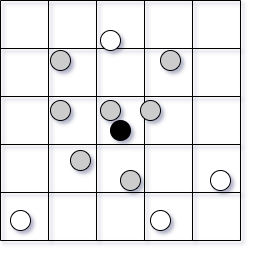
\includegraphics[width=0.99\linewidth]{neib_grid.drawio}
        \caption{
            Graficzna reprezentacja działania siatki sąsiedztwa.
        }
    \end{wrapfigure}

    Siatka sąsiedztwa minimalizuje liczbę obliczeń kolizji pomiędzy węzłami 
    należącymi do różnych obiektów. Jest on bardzo potrzebny do utrzymania 
    pożądanej prędkości wykonywania symulacji w przypadkach gdy składa się ona 
    z dużej liczy obiektów, które mogą ze sobą potencjalnie kolidować. \\
    
    Na podstawie znajdującego się po prawej stronie rysunku można łatwo opisać
    działanie tego algorytmu. Z perspektywy czarnego węzła
    potencjale kolizje między nim a innymi węzłami mogą wystąpić tylko 
    jeżeli środek innego węzła znajduje się w tej 
    samej komórce co on lub w komórce sąsiadującej z jego komórką. Na rysunku 
    węzły z którymi sprawdzona będzie kolizja z węzłem czarnym oznaczone zostały
    kolorem szarym. Węzły które nie znajdują się w branych pod uwagę komórkach 
    zostaną zignorowane podczas obliczeń, zostały one oznaczone kolorem białym. \\

    Kroki jakie należy wykonać w celu wykorzystania siatki sąsiedztwa na 
    potrzeby symulacji fizycznej prezentują się następująco:
    \begin{enumerate}
        \item Tworzymy tablicę pustych dynamicznych wektorów, jeden wektor dla każdej komórki siatki.

        \item Iterujemy po wszystkich węzłach i mapujemy położenie węzła na komórkę. Wpisujemy indeks węzła 
        do wektora zawartego w komórce. W tym kroku możemy również zastosować inne optymalizacje, jak na przykład 
        ignorowanie węzłów które nie są węzłami brzegowymi danego obiektu.

        \item Gdy chcemy obliczyć nowe przyśpieszenie dla węzła, bierzemy pod uwagę tylko węzły znajdujące 
        się w tej samej lub sąsiadującej komórce.
    \end{enumerate}

    Siatka musi być często aktualizowana aby zapewnić odpowiednie wyniki. W raz z upływem czasu symulacji położenia
    węzłów będą się zmieniać, nieodpowiednio utrzymywana siatka sąsiedztwa może doprowadzić do zignorowania 
    oddziaływania pomiędzy węzłami znajdującymi się blisko siebie. W projekcie siatka budowana jest od nowa 
    co kilka iteracji symulacji.
    
    \clearpage
    \begin{wrapfigure}{R}{0.5\textwidth}
        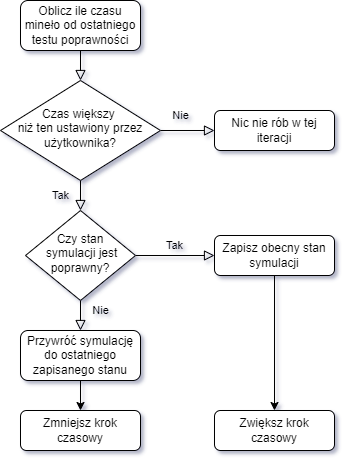
\includegraphics[width=0.95\linewidth]{error_correction.drawio.png}
        \caption{
            Schemat blokowy przedstawiający sposób działania
            algorytmu sprawdzającego co klatkę
            błędy w symulacji i zarządzającego wartością kroku czasowego
        }
    \end{wrapfigure}

    \subsection{Korekta błędów}
    Z powodu dobrania zbyt dużego kroku czasowego symulacja może być niestabilna.
    Objawy niestabilności to między innymi destrukcja siatki, nadanie węzłów 
    ogromnych prędkości powodujących wyjście poza obserwowalny obszar.
    Zaczynają występować niepoprawne wartości odległości take jak \emph{nan} lub \emph{inf}.
    Gdy takie wartości się pojawią obecny stan uznany jest niepoprawny i symulacja wraca 
    do ostatniego zapisanego stanu w którym 
    te wartości nie występowały. Co pewien czas tworzona jest nowa kopia zapasowa.

    Jeżeli stan symulacji jest poprawny zapisuje go do pamięci, jeżeli nie jest on poprawny to symulacja 
    przywracana jest do ostatniego poprawnego stanu a krok czasowy jest zmniejszany.

    \subsection{Automatyczny dobór kroku czasowego}
    Gdy korekta błędów jest włączona za każdym razem gdy zostanie wykryty błąd i powrót do poprzedniego stanu
    krok czasowy zostanie zmniejszony o połowę. Jeżeli użytkownik włączy funkcję automatycznego zwiększania
    kroku czasowego, krok czasowy będzie przemnażany przez wybraną przez użytkownika wartość większą od 
    jeden za każdym razem gdy podczas tworzenia nowej kopii nie zostanie wykryty błąd. \\ \\ \\ \\
    
    Efektywnie działanie tego algorytmu jest bardzo proste, jeżeli wykryjemy błąd zmniejszamy krok czasowy
    przez co symulacja wykonuje się dłużej i dokładniej, co znacząco zmniejsza ryzyko, że błąd
    ten wystąpi ponownie. Jednocześnie jeżeli błąd nie został wykryty możemy spróbować zwiększyć 
    krok czasowy, wykonując symulację mniej dokładnie ale za to skracając czas obliczeń.

    % ---------------------------------------------------------------------------------------------------
    \clearpage
    \section{Generowanie grafiki}
    Do generowania grafiki i animacji został wykorzystany \emph{\emph{OpenGL}}, 
    wielojęzyczny i wieloplatformowy 
    interfejs programowania aplikacji do renderowania grafiki wektorowej 2D i 3D, 
    od 2006 roku zarządzany przez konsorcjum technologiczne non-profit Khronos Group. 
    Interfejs API jest zwykle używany do interakcji 
    z procesorem graficznym w celu uzyskania renderowania z przyspieszeniem sprzętowym. 
    Specyfikacja \emph{OpenGL} opisuje abstrakcyjne API do rysowania grafiki 2D i 3D. Chociaż możliwe jest 
    zaimplementowanie API w całości programowo, jest ono zaprojektowane do implementacji głównie 
    lub całkowicie sprzętowej.

    Ten interfejs programowania zdefiniowany jako zestaw funkcji, które mogą być wywoływane przez program.
    Chociaż definicje tych funkcji są podobne do tych z języka programowania \emph{C}, to tak 
    naprawdę są one niezależne od języka od jakiegokolwiek języka. 
    \emph{OpenGL} jest również wieloplatformowy przez co programy go wykorzystujące mogą 
    działać poprawnie na systemie operacyjnym Windows jak i systemach z rodziny Linux. 
    Specyfikacja nie mówi nic na temat uzyskiwania i zarządzania kontekstem \emph{OpenGL}, 
    pozostawiając to systemowi okien; \emph{OpenGL} zajmuje się wyłącznie 
    renderowaniem, nie dostarczając żadnych interfejsów API związanych z wejściem, dźwiękiem lub oknami. \\

    Na cele aplikacji wykorzystane zostało API \emph{OpenGL} w \emph{profilu rdzennym} (core profile), 
    pozwalającym samodzielnie programować \emph{shadery} (programy działające na procesorze graficznym, 
    zazwyczaj odpowiedzialne za ustalenie pozycji werteksów lub obliczenie koloru piksela) \cite{grafika3d}, 
    co w diametralny sposób zmienia w jaki sposób pisane są programy graficzne w porównaniu 
    do starszych wersji \emph{OpenGL}, znacznie zwiększając możliwości programistów z niego 
    korzystających. W nowoczesnym \emph{OpenGL} potok renderowania składa 
    się z następujących kroków \cite{grafika3d}:
    \begin{enumerate}
        \item Stworzenia buforów na werteksy i indeksy.
        \item W shaderze werteksów przekształcenia położeń werteksów 
        za pomocą macierzy rzutowania i ustalenia koloru dla każdego werteksu.
        \item Przycinanie i rasteryzacja.
        \item Shader fragmentów wykonuje operacje na pikselach mających na celu 
        ustalenie ostatecznego koloru dla każdego piksela.
        \item Test głębi, blending.
    \end{enumerate}

    Macierz rzutowania odpowiada za transformację z układu współrzędnych kamery do \emph{układu przycinania}
    (clip coordinate system) \cite{grafika3d}. W aplikacji 
    zaimplementowana została kamera która pozwala na przemieszczanie się po scenie i jest również w stanie 
    przybliżać i oddalać obraz. 
    Ponieważ przestrzeń po której porusza się
    kamera jest dwuwymiarowa, macierz taka ma wymiary $3 \times 3$, o jeden wymiar więcej niż wymiarowość 
    przestrzeni, aby poza zwykłymi transformacjami takimi jak rotacja czy skala, uwzględnić również
    translację (przemieszczenie).
    W ten sposób zaimplementowana kamera daje duże możliwości użytkownikowi programu, pozwalając 
    mu na obserwowanie dowolnego miejsca w przestrzeni jednocześnie dając mu możliwość zwiększania
    lub zmniejszania wielkości obserwowanych obiektów. \\

    Oczywiście podczas projektowania aplikacji graficznej należy również zadbać o
    wydajność rysowania obiektów. Nawet proste użycie stałego bufora zamiast jego 
    zmiennego odpowiednika może wyraźnie skrócić czas rysowania.
    Inną istotną optymalizacją zastosowaną w aplikacji jest użycie 
    metody \emph{renderowania instancjonowanego} (instanced rendering), 
    metoda pozwalająca na renderowanie wielu obiektów na raz 
    przy użyciu jednego wywołania funkcji rysującej (draw call). 
    Najpierw należy zainicjalizować geometrię obiektu który będzie renderowany, 
    następnie stworzyć tablicę zwierającą informację 
    między innymi o położeniu każdego z tych obiektów. 
    W ten sposób zamiast rysować każdy obiekt w osobnym wywołaniu, 
    możemy narysować wszystkie obiekty jednocześnie, 
    w ten sposób wyraźnie zwiększając wydajność programu.

    % --------------------------------------------------------------------------------------------------------------
    \clearpage
    \section{Widok aplikacji}
    Program ma formę aplikacji okienkowej. Na ekranie widoczny jest aktualny stan symulacji wraz z 
    panelami ustawień zawierającymi interaktywne kontrolki pozwalające zmieniać na 
    bieżąco parametry symulacji i sposób jej wyświetlania. Aplikacja jest kompatybilna z
    systemami operacyjnymi z rodzin Windows i Linux.

    \begin{figure}[H]
        \centering
        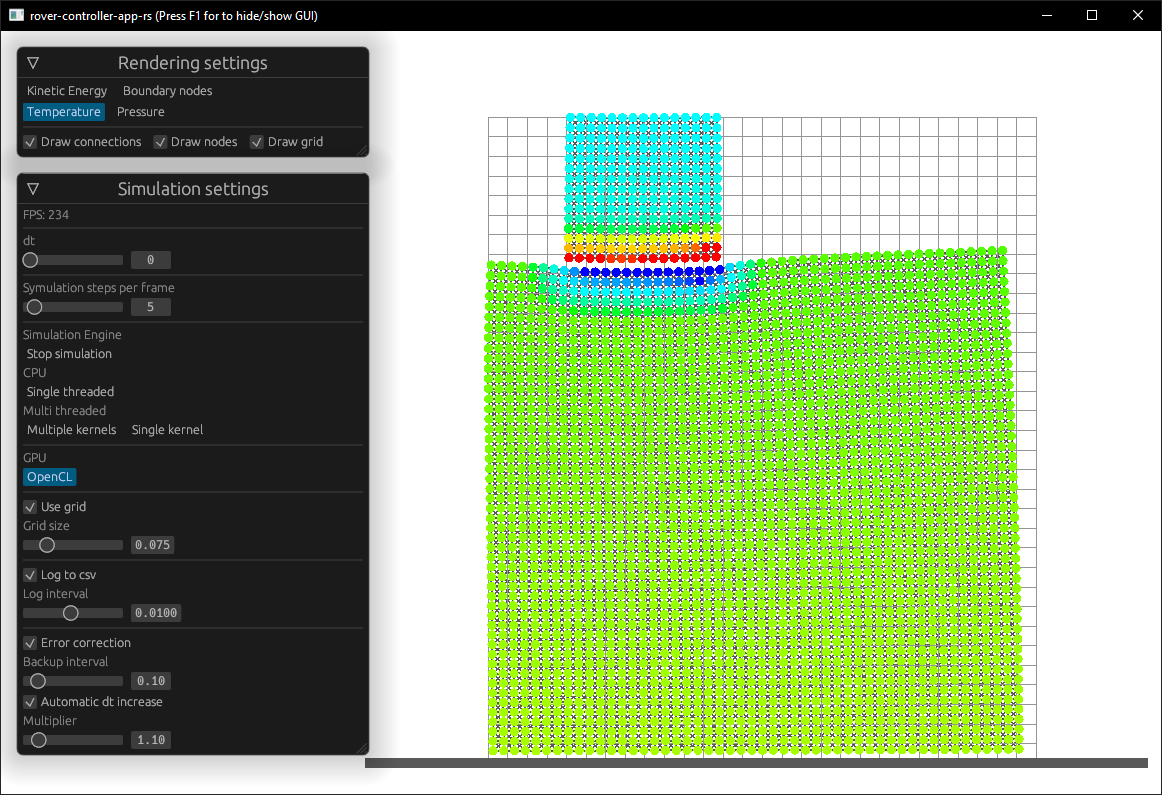
\includegraphics[width=17cm]{app_view_full.png}
        \caption{
            Okno aplikacji z widocznymi panelami ustawień
            w systemie operacyjnym Windows.
        }
    \end{figure}
    
    Widoczne po lewej stronie panele można ukryć lub ponownie wyświetlić klikając
    przycisk funkcyjny \emph{F1} na klawiaturze. Za pomocą myszy można zmieniać położenie kamery, 
    co pozwala na wybranie i obserwowanie konkretnego, interesującego nas obszaru symulacji.
    Samo przybliżenie kamery również jest konfigurowalne; za pomocą rolki myszy możemy oddalać 
    lub przybliżać kamerę, co daje nam dużą dowolność podczas analizy stanu symulacji.

    \subsection{Opcje symulacji}
    Użytkownik może w dowolnym momencie trwania symulacji zmienić niektóre z jej parametrów:
    \begin{enumerate}
        \item \emph{Krok czasowy} - wartość kroku czasowego można ustawić za pomocą suwaka lub też wpisać
        ją ręcznie w dostępnym polu.

        \item \emph{Ilość kroków symulacji na wyświetlaną klatkę} - wartość określa ilość kroków symulacji

        \item \emph{Silnik symulacji} - pozwala zmieniać sposób w jaki obliczane są kolejne kroki symulacji.
        Można wybrać pomiędzy symulowaniem za pomocą CPU jedno lub wielowątkowo, gdzie dostępne są dwa
        tryby wielowątkowe. Można również wybrać tryb symulacji za pomocą GPU, gdzie wykorzystywane jest API OpenCL.

        \item \emph{Siatka sąsiedztwa} - można wybrać czy obliczanie kolizji ma być przyśpieszone przez użycie
        siatki sąsiedztwa.

        \item \emph{Zapisywanie logów do pliku csv} - pozwala zapisywać logi zawierające informacje o stanie
        energii symulacji w danych chwilach czasowych do pliku CSV. Można określić częstotliwość zapisywania
        za pomocą suwaka. Opcja ta znacznie wpływa na wydajność, dlatego jest domyślnie wyłączona.

        \item \emph{Korekcja błędów} - co pewien czas sprawdza czy symulacja nie uległa degradacji i 
        w razie potrzeb przywraca ją do poprawnego stanu.

        \item \emph{Automatyczny dobór kroku czasowego} - opcja dostępna jedynie gdy korekcja błędów jest włączona.
        Za każdym razem gdy nie zostanie wykryty błąd podczas zapisywania stanu symulacji, krok czasowy zostaje
        pomnożony przez wartość którą można dowolnie zmieniać za pomocą suwaka.
        
    \end{enumerate}

    \begin{figure}[H]
        \centering
        \begin{subfigure}[t]{0.4\textwidth}
            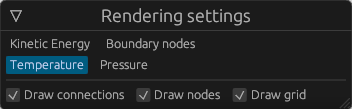
\includegraphics[width=\textwidth]{render_settings.png} 
            \caption{Panel ustawień rysowania}
        \end{subfigure}
        \begin{subfigure}[t]{0.4\textwidth}
            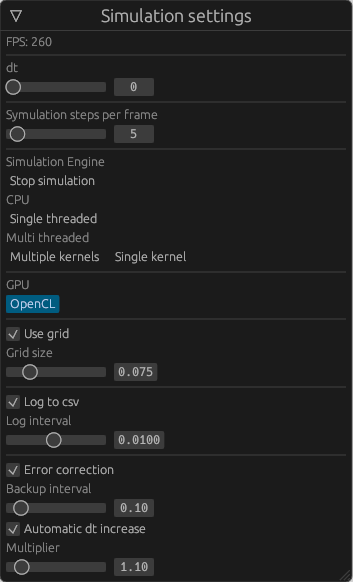
\includegraphics[width=\textwidth]{simulation_settings.png}
            \caption{Panel ustawień symulacji}
        \end{subfigure}
        \caption{Widok paneli ustawień dostępnych w aplikacji}
    \end{figure}

    Panele ustawień można ustawić w dowolnym miejscu w oknie aplikacji, przeciągając je za pomocą myszy.
    Każdy z paneli można również zwinąć lub rozwinąć klikając na trójkąt znajdujący się po lewej 
    stronie paska tytułowego każdego z paneli.

    \clearpage
    \subsection{Dostępne tryby rysowania}
    Funkcje rysowania \emph{połączeń węzłowych}, \emph{węzłów} i \emph{siatki obliczeniowej} domyślnie 
    jest włączone ale można w każdej chwili wyłączyć dowolną z nich korzystając z panelu ustawień rysowania.
    Węzły można kolorować na następujące sposoby:

    \begin{enumerate}
        \item \emph{Energia kinetyczna} - kolorujemy węzły na podstawie ich energii kinetycznej 
        gdzie kolor czarny to zerowa energia kinetyczna, wraz z jej zwiększaniem węzeł staje się czerwony.

        \item \emph{Węzły brzegowe} - węzły brzegowe danego obiektu mają ten sam kolor,
        każdy obiekt ma inny kolor węzłów brzegowych. Węzły wewnętrzne każdego z obiektów są koloru szarego.

        \item \emph{Temperatura} - każdy węzeł otrzymuje kolor zależy od jego temperatury. 
        Skala kolorów zaczyna się od ciemno-niebieskiego dla najniższych wartości, 
        przechodzi w zielony, żółty, pomarańczowy a węzły o kolorze czerwonym
        cechują się najwyższą wartością temperatury.

        \item \emph{Ciśnienie} - każdy węzeł otrzymuje kolor zależy od jego ciśnienia. 
        Skala kolorów jest analogiczna do tej występującej przy wyświetlaniu temperatury.
    \end{enumerate}

    \begin{figure}[h]

        \begin{subfigure}{0.5\textwidth}
            \centering
            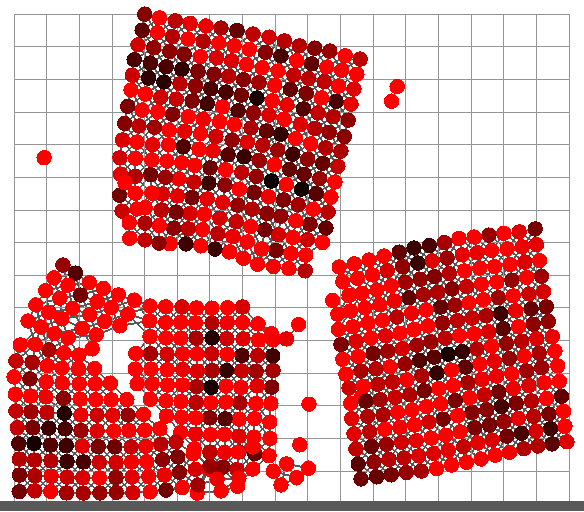
\includegraphics[width=6cm]{app_kinetic_view.png} 
            \caption{Energia kinetyczna}
        \end{subfigure}
        \begin{subfigure}{0.5\textwidth}
            \centering
            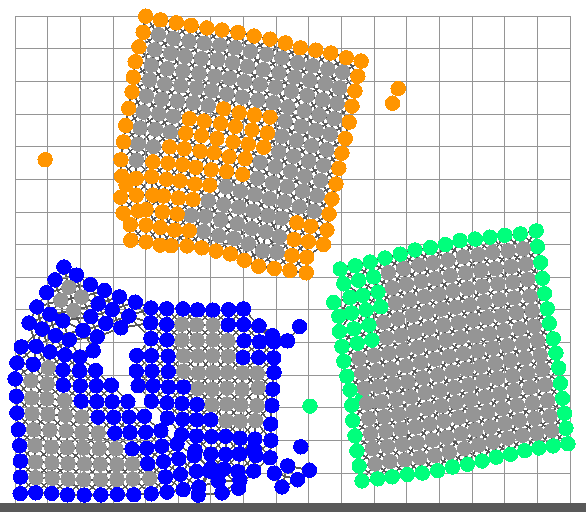
\includegraphics[width=6cm]{app_boundary_view.png}
            \caption{Węzły brzegowe}
        \end{subfigure}
        \begin{subfigure}{0.5\textwidth}
            \centering
            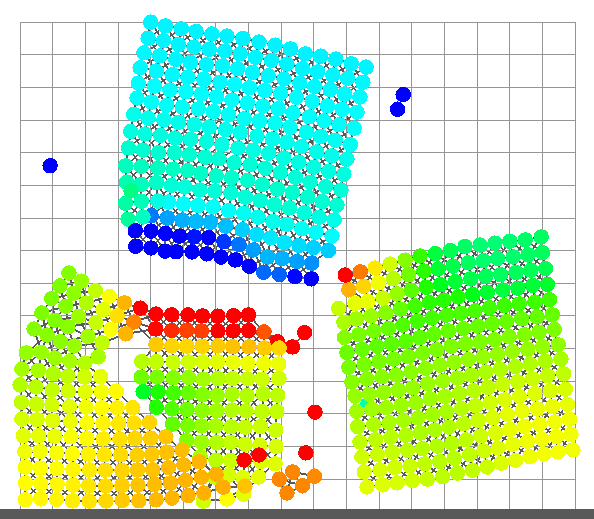
\includegraphics[width=6cm]{app_temperature_view.png}
            \caption{Temperatura}
        \end{subfigure}
        \begin{subfigure}{0.5\textwidth}
            \centering
            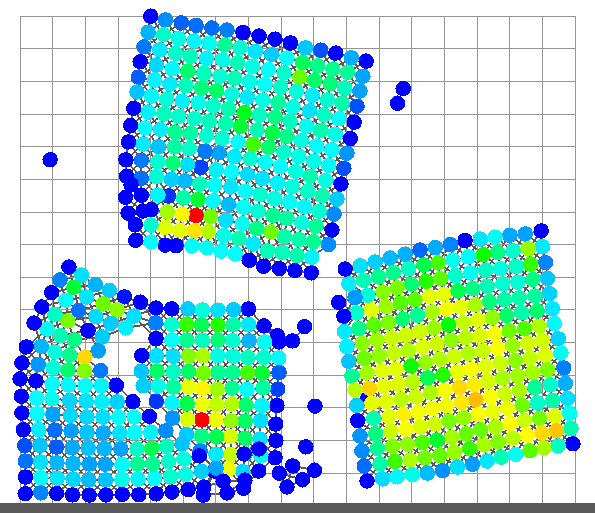
\includegraphics[width=6cm]{app_pressure_view.png}
            \caption{Ciśnienie}
        \end{subfigure}
        
        \caption{Porównanie widoków z tej samej sceny w czterech trybach kolorowania węzłów.}
    \end{figure}

\chapter{Testy}
    \section{Test poprawności działania algorytmów}
    \subsection{Opis testu}
    
    \begin{wrapfigure}{r}{0.45\textwidth}
        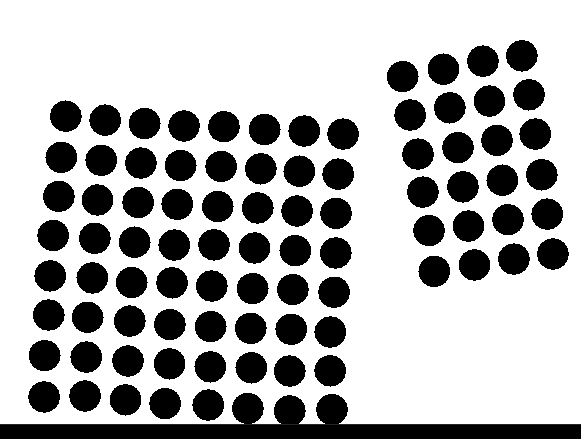
\includegraphics[width=0.9\linewidth]{objects_raw} 
        \caption{Widok aplikacji z widocznymi dwoma obiektami $8 \times 8$ oraz $6 \times 4$}
    \end{wrapfigure}
    Jeżeli wszystkie algorytmy symulujące oddziaływania fizyczne zostały zaimplementowane poprawnie 
    to w przypadku gdy nie występują żadne siły oporu energia całkowita układu powinna 
    być stała przez cały czas trwania symulacji. Aby uzyskać poprawny obraz sytuacji należy 
    uwzględnić wszystkie rodzaje energii w układzie: 
    \begin{enumerate}
        \item Energia potencjalna grawitacji
        \item Energia kinetyczna
        \item Energia potencjalna wewnątrz obiektu
        \item Energia potencjalna odpychająca pomiędzy obiektami a podłożem
        \item Energia potencjalna odpychająca pomiędzy dwoma obiektami
    \end{enumerate}

    Do testu zachowania energii wykorzystane są dwa obiekty o rozmiarach 
    odpowiednio $8 \times 8$ i $6 \times 4$ oraz statyczne podłoże. Obiekty
    znajdują się w polu grawitacyjnym, nie ma żadnych sił oporu/tarcia.

    \subsubsection{Parametry symulacji}
    \begin{align*}
        g &= 9.81 [\frac{m}{s^2}] \\
        dt &= 10^{-5} [s] \\
        t_{max} &= 8 [s] \\
        n = \frac{t_{max}}{dt} &= 8 \times 10^{5}
    \end{align*}

    \subsection{Wyniki}
    \begin{figure}[H]
        \centering
        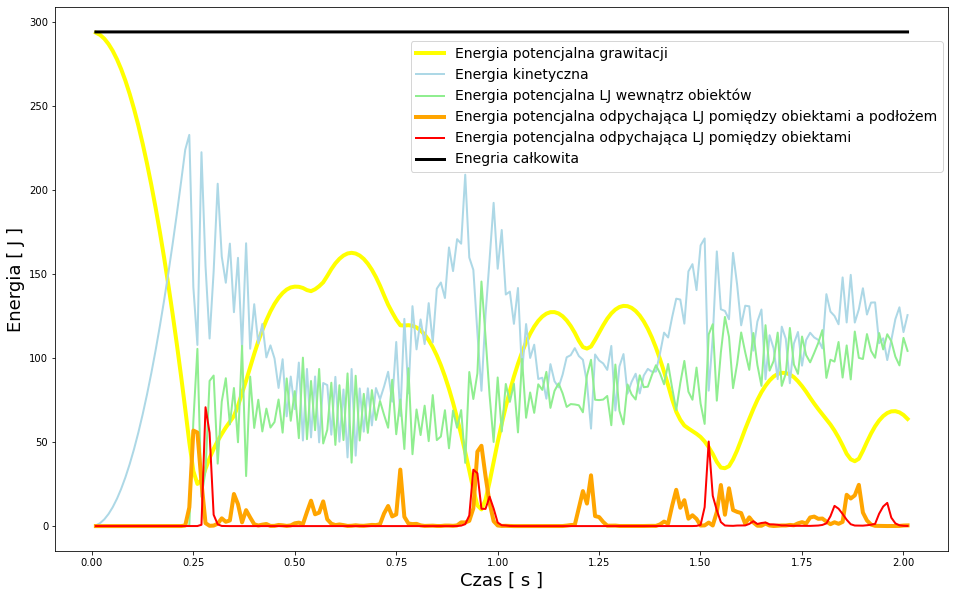
\includegraphics[width=14cm]{energy_test_0to2s}
        \caption{Zmiana energii w czasie dla układu w ciągu pierwszych 1.2 sekund}
    \end{figure}


    W początkowej fazie testu wyżej zawieszony obiekt zaczyna spadać
    pod wpływem siły ciążenia na stacjonarny drugi obiekt znajdujący
    się przy podłożu. Po nieco ponad $0.2 [s]$ dochodzi do pierwszego kontaktu.
    Przy zderzeniach pomiędzy obiektami oraz pomiędzy obiektem i podłożem energia potencjalna
    odpychająca Lennarda-Jonesa oznaczona kolejno kolorami pomarańczowym i czerwonym
    wyraźnie wzrasta. Zaraz po zderzeniu możemy obserwować ponowny wzrosty energii potencjalnej grawitacji,
    gdyż obiekt $6 \times 4$ wykorzystując obiekt $8 \times 8$ jako trampolinę ponownie wznosi się na 
    pewną wysokość, która jest jednak wyraźnie niższa od poprzedniej.

    \begin{figure}[H]
        \centering
        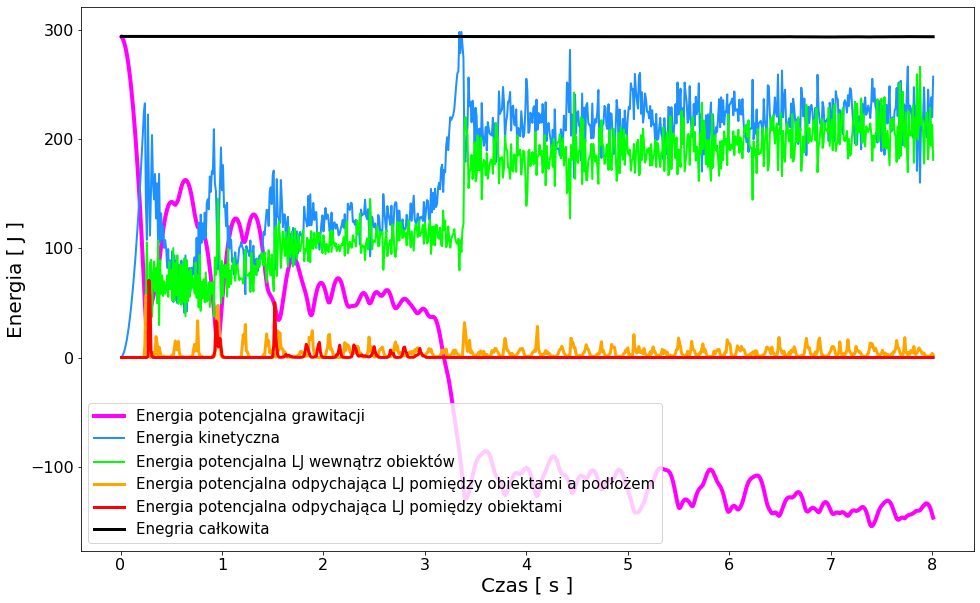
\includegraphics[width=14cm]{energy_test_0to8s}
        \caption{Zmiana energii w czasie dla układu w ciągu pierwszych 8 sekund}
    \end{figure}
    
    Obiekt $6 \times 4$ odbija się jeszcze kilkukrotnie od obiektu $8 \times 8$, za każdym 
    razem na nieco mniejszą wysokość, przez co następuje utrata energi potencjalnej grawitacji 
    na rzecz energii wewnętrznych obydwóch obiektów. Po nieco ponad $3.0 [s]$ obiekt 
    $6 \times 4$ zsuwa sie z drugiego obiektu i spada na podłoże

    \begin{figure}[H]
        \begin{subfigure}{0.5\textwidth}
            \centering
            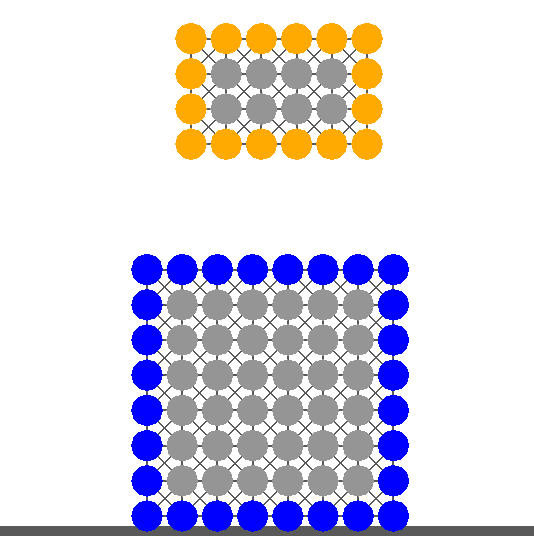
\includegraphics[width=5.5cm]{app_correctness_01.png} 
            \caption{Stan początkowy}
        \end{subfigure}
        \begin{subfigure}{0.5\textwidth}
            \centering
            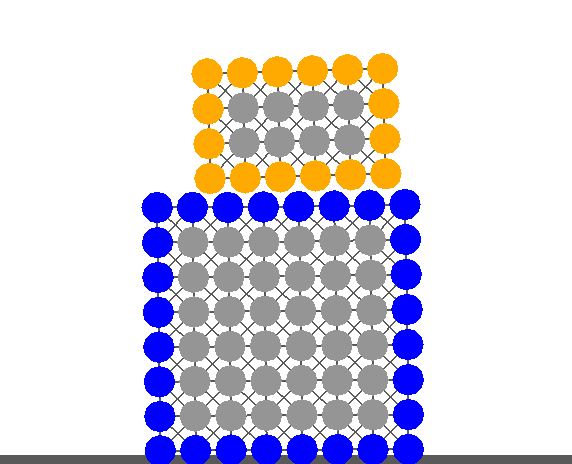
\includegraphics[width=6cm]{app_correctness_02.png}
            \caption{Pierwsze zderzenie}
        \end{subfigure}
        \begin{subfigure}{0.5\textwidth}
            \centering
            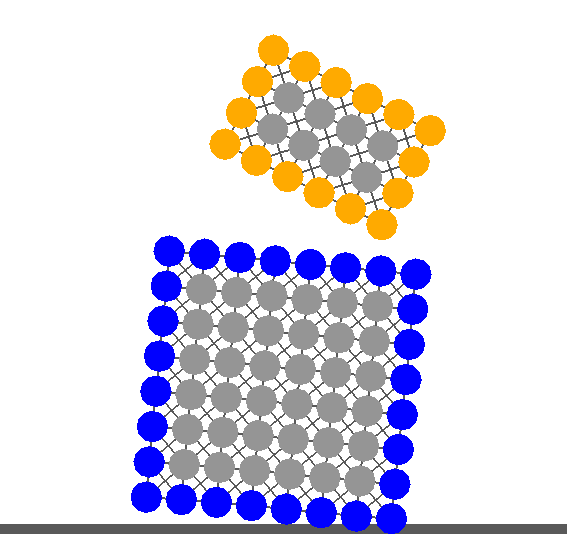
\includegraphics[width=6cm]{app_correctness_03.png}
            \caption{Kilkukrotne odbijanie się obiektów}
        \end{subfigure}
        \begin{subfigure}{0.5\textwidth}
            \centering
            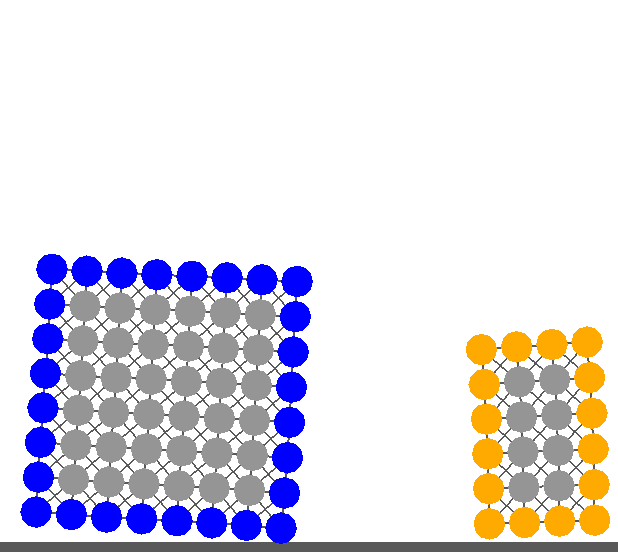
\includegraphics[width=6.3cm]{app_correctness_04.png}
            \caption{Zsunięcie się z siebie obiektów}
        \end{subfigure}
        
        \caption{Widok aplikacji podczas wykonywania testu poprawności działania algorytmów.}
    \end{figure}

    Po upłynięciu kilku sekund obiekty zostają przy podłożu, energia będąca początkowo energią
    potencjalną grawitacji została w większości zamieniona na energię kinetyczną oraz energię
    wewnętrzną. Obiekty nie odbijają się one już między sobą.
    Zmiana energii całkowitej w czasie działania całej symulacji była mniejsza niż $1\%$. Na tej
    podstawie można uznać, że algorytmy zostały zaimplementowane poprawnie.

    \clearpage
    % --------------------------------------------------------------------------------------------------------------
    \section{Test wydajności dla dwóch algorytmów obsługi zderzeń między obiektami}
    \subsection{Opis algorytmów}
    Naszym celem jest obliczanie siły pomiędzy odpowiednimi węzłami w taki sposób aby 
    obiekty przy zderzeniu odpychały się od siebie.
    
    \begin{figure}[h]
        \centering
        \begin{subfigure}[t]{0.4\textwidth}
            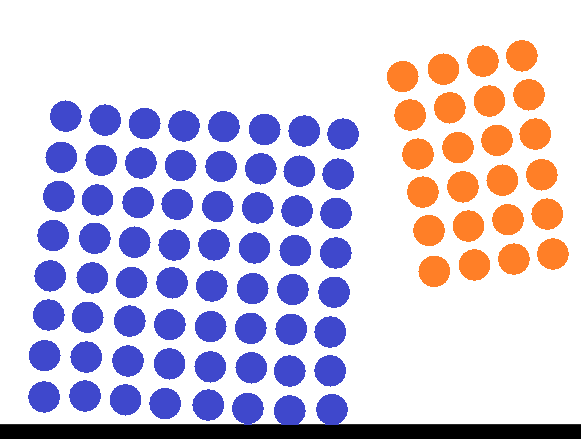
\includegraphics[width=\textwidth, height=6cm]{objects_unoptimized} 
            \caption{Każdy węzeł jednego obiektu z każdym każdym węzłem drugiego obiektu}
        \end{subfigure}
        \begin{subfigure}[t]{0.4\textwidth}
            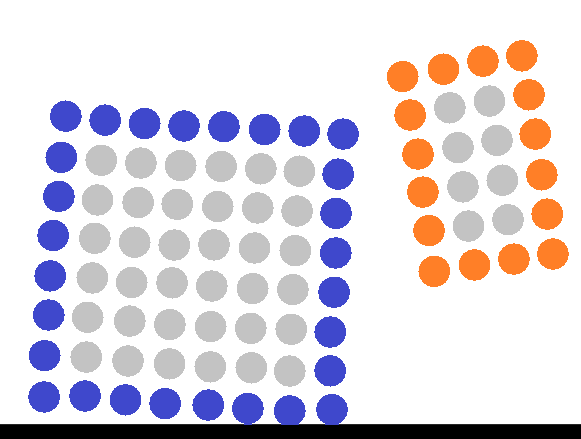
\includegraphics[width=\textwidth, height=6cm]{objects_optimized}
            \caption{Węzły zewnętrzne jednego obiektu z węzłami zewnętrznymi drugiego obiektu}
        \end{subfigure}
        \caption{Reprezentacja dwóch metod obsługi zderzeń}
    \end{figure}

    Dla metody (a) oddziaływanie liczone jest pomiędzy każdym węzłem o kolorze niebieskim z każdym węzłem o
    kolorze pomarańczowym. Metoda o złożoności $O(n^2)$ gdzie $n$ to liczba węzłów.
    Jest to metoda bardzo wolna, lecz dająca poprawne rezultaty w każdym symulowanym przypadku.\\

    Dla metody (b) oddziaływanie ponownie liczone jest pomiędzy każdym węzłem o kolorze niebieskim z każdym
    węzłem o kolorze pomarańczowym, tym razem jednak oznaczone są jedynie węzły brzegowe.
    Metoda ta jest szczególnie efektywna dla obiektów kwadratowych o boku $n$, gdzie z $n^2$
    rozpatrywanych węzłów ta liczba jest zmniejszona do zaledwie $4(n-1)$ węzłów.
    Należy zwrócić uwagę, że metoda ta nie będzie poprawnie odwzorowywać oddziaływań dla
    obiektów zagnieżdżonych w sobie. Przykładowa sytuacja, w której algorytm nie zadziała poprawnie
    to symulacja penetracji/rozrywania obiektów - poprawna obsługa tego przypadku wymagała by odpowiedniej
    modyfikacji brzegów obiektów.

    \subsection{Opis testu}
    Rozpatrujemy scenariusz z dwoma obiektami, sprawdzamy liczbę iteracji symulacji na sekundę stopniowo
    zwiększając liczbę węzłów w obydwóch obiektach.
    Test wydajności został wykonany na procesorze \emph{AMD Ryzen 5 5600X}, 
    jest to jednowątkowa wersja algorytmu działająca na CPU.
    Ilość węzłów w bokach obiektów ustawiana jest kolejno na: 
    3, 5, 9, 10, 15, 21, 25, 30, 35, 40, 45, 50, 55, 60. Parametry symulacji dobrane są 
    w taki sposób, aby obiekty nie uległy uszkodzeniu/rozerwaniu.
    
    \subsection{Wyniki}
    Wyniki z przeprowadzonego testu prezentują się następująco:
    \begin{figure}[H]
        \centering
        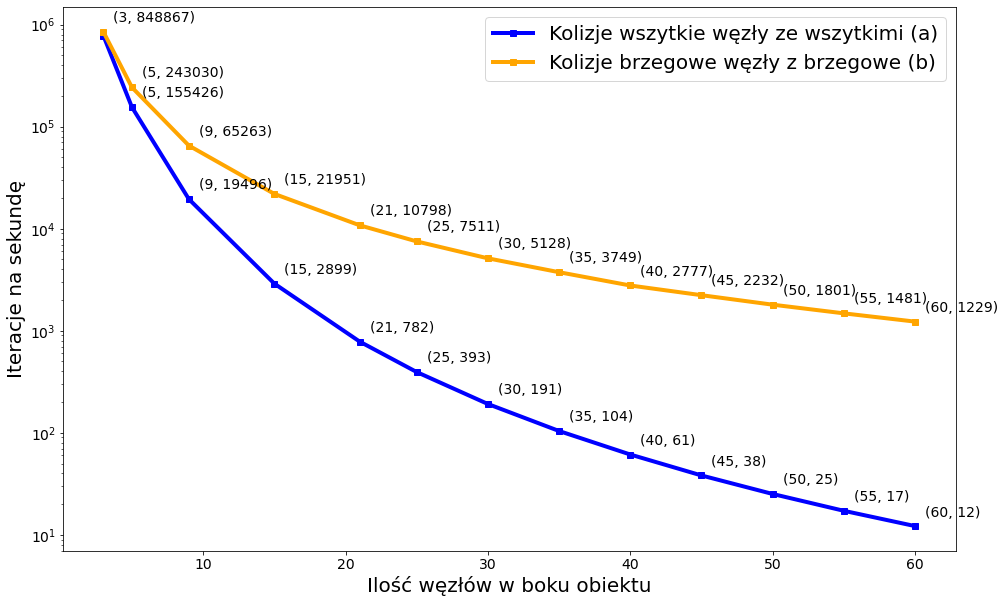
\includegraphics[width=16cm]{performance_side_size}
        \caption{
            Liczba iteracji na sekundę w zależności od 
            ilości węzłów w bokach obiektów dla dwóch metod obsługi zderzeń -
            oś iteracji na sekundę jest przedstawiona w skali logarytmicznej.
        }
    \end{figure}

    \begin{figure}[H]
        \centering
        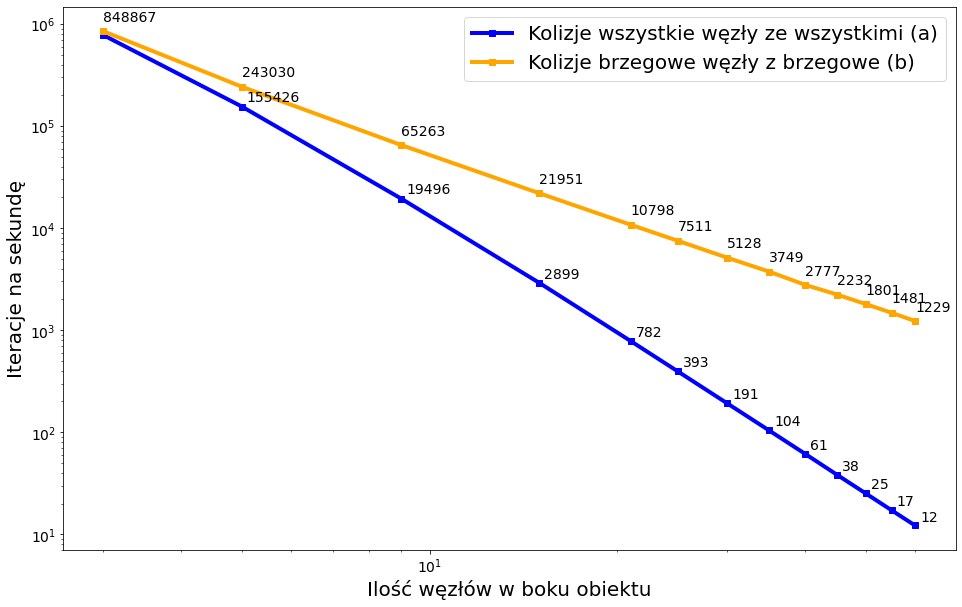
\includegraphics[width=16cm]{performance_side_size_log_log}
        \caption{
            Liczba iteracji na sekundę w zależności od 
            ilości węzłów w bokach obiektów dla dwóch metod obsługi zderzeń -
            oś iteracji na sekundę i oś liczby węzłów w boku obiektu są przedstawione w skali logarytmicznej.
        }
    \end{figure}

    \begin{table}[H]
        \centering
        \begin{tabular}{||c c c c||} 
            \hline
            węzły w boku obiektu & $iteracje / [s]$ dla (a) & $iteracje / [s]$ dla (b) & krotność przyśpieszenia \\ [0.5ex] 
            \hline\hline
            3 & 777633 & 848867 & 1.09 \\ 
            \hline
            5 & 155426 & 243030 & 1.56 \\
            \hline
            9 & 19496 & 65263 & 3.34 \\
            \hline
            15 & 2899 & 21951 & 7.57 \\
            \hline
            21 & 782 & 10798 & 13.79 \\
            \hline
            25 & 393 & 7511 & 19.06 \\
            \hline
            30 & 191 & 5128 & 26.76 \\
            \hline
            35 & 104 & 3749 & 36.00 \\
            \hline
            40 & 61 & 2777 & 45.33 \\ 
            \hline
            45 & 38 & 2232 & 58.43 \\ 
            \hline
            50 & 25 & 1801 & 71.63 \\
            \hline
            55 & 17 & 1481 & 86.11 \\ 
            \hline
            60 & 12 & 1229 & 100.88 \\ [1ex] 
            \hline
        \end{tabular}
        \caption{ Porównanie wydajności przypadku niezoptymalizowanego (a) i zoptymalizowanego (b) }
    \end{table}
    Dla większych obiektów zyski z zastosowanej optymalizacji są bardzo duże, w przypadku dwóch obiektów
    $60 \times 60$ ilość iteracji dla algorytmu zoptymalizowanego jest ponad $100$ razy większa.

    Wzrost wydajności można łatwo zobrazować rozpatrując jeden z przypadków. Gdy rozważymy dwa 
    obiekty kwadratowe $60 \times 60$ daje nam to $3600$ węzłów na obiekt.
    Dla wersji niezoptymalizowanej mamy $3600 \times 3600 = 12960000$ operacji, natomiast wersja druga to zaledwie
    $4(n - 1) \times 4(n - 1) = 4(60 - 1) \times 4(60 - 1) = 236 \times 236 = 55696$ operacji. Oznacza to, że 
    w wersji każdy węzeł z każdym węzłem dla tego konkretnego przypadku musimy wykonać ponad $232$ razy więcej obliczeń
    kolizji między obiektami, gdzie zdecydowana większość z nich ma zaniedbywalny efekt na działanie symulacji. \\

    Warto zwrócić uwagę na to, że pomimo redukcji ponad $232$ razy obliczeń dla kolizji, 
    liczba wykonanych iteracji na sekundę dla przypadku dwóch obiektów $60 \time 60$ wzrosła jedynie
    nieco ponad stukrotnie. Wynika to z faktu, że optymalizacja ta obejmuje jedynie etap obliczania
    kolizji między różnymi obiektami i nie wpływa na obliczanie interakcji w tym samym obiekcie,
    obliczanie wpływu pola grawitacyjnego czy obliczanie wpływu sił oporu.
    
    \clearpage
    % --------------------------------------------------------------------------------------------------------------
    \section{Testy wydajności algorytmów z rozrywaniem obiektów}
    \begin{wrapfigure}{r}{0.4\textwidth}
        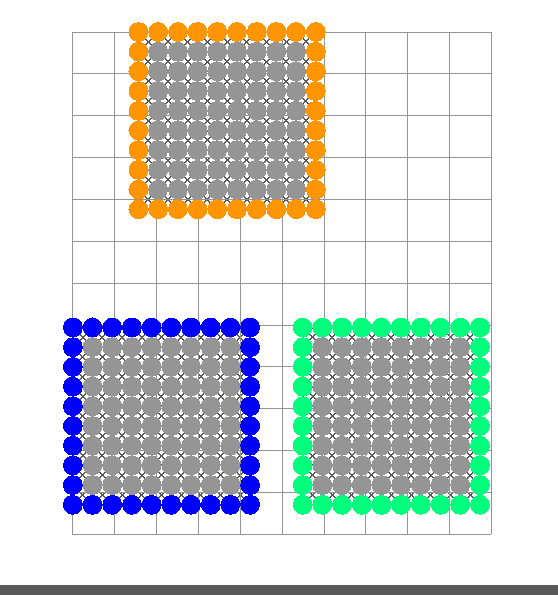
\includegraphics[width=0.9\linewidth]{app_boundary_performance_10x10_01.png} 
        \caption{Stan początkowy dla sceny z obiektami $10\times10$}
        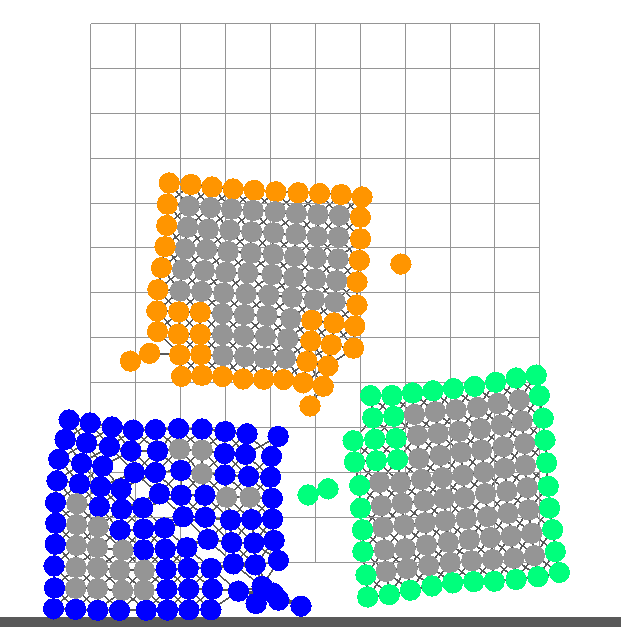
\includegraphics[width=0.9\linewidth]{app_boundary_performance_10x10_02.png} 
        \caption{Zderzenie i rozerwaniu obiektów $10\times10$}
    \end{wrapfigure}
    \subsection{Opis testu}
    Scena składa się z trzech obiektów zawieszonych nad podłożem na różnych wysokościach. Siła grawitacji 
    powoduje swobodny spadek tych obiektów a następnie zderzanie się i ich rozrywanie. Liczba węzłów jest
    stopniowo zwiększana poprzez zwiększanie gęstości każdego z trzech obiektów. W układzie nie
    występują żadne siły oporu ruchu.\\
    
    Ilość węzłów w boku 
    każdego z tych obiektów wynosi kolejno 5, 10, 15, 25, 40, 50, 60, 75, 90, 100. Dla 
    testów najwydajnejszych algorytmów dla CPU i GPU zostały wykonane dodatkowe testy z 
    bardzo gęstymi obiektami, liczba węzłów w bokach tych obiektów wynosi kolejno 150, 200, 250, 300.
    Testy wydajności został wykonany na procesorze \emph{AMD Ryzen 5 5600X} i
    karcie graficznej Nvidia RTX 3060. \\
    
    Krok czasowy symulacji wynosi
    $2 \times 10^{-5}$ sekundy a czas trwania symulacji to $0.5$ sekundy, co 
    daje $25000$ kroków symulacji dla każdego przypadku. \\

    \clearpage
    % --------------------------------------------------------------------------------------------------------------
    \subsection{Test wydajności z węzłami brzegowymi}
    \begin{figure}[H]
        \centering
        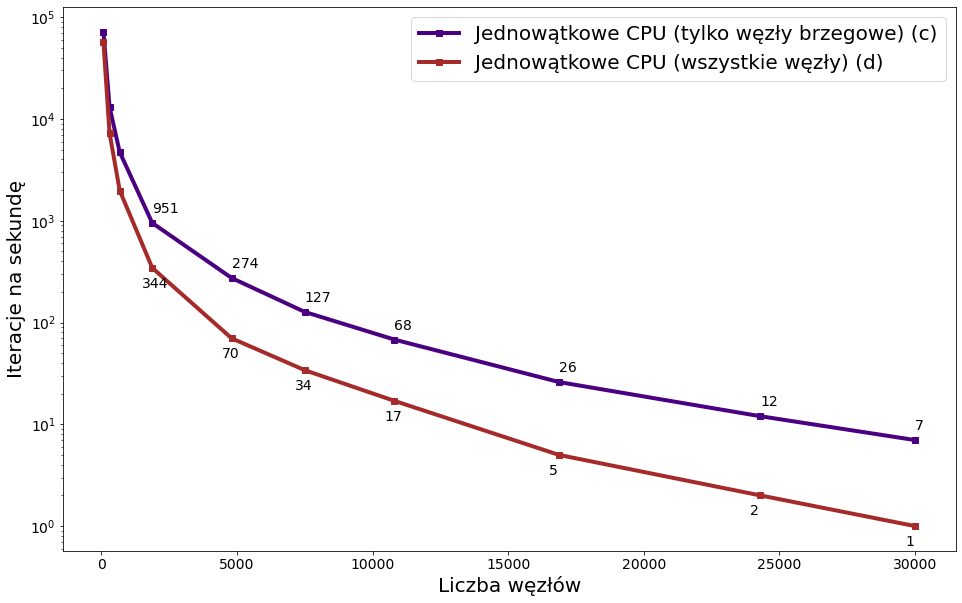
\includegraphics[width=18cm]{performance_cpu_boundary_noboundary.png}
        \caption{
            Liczba iteracji na sekundę w zależności od ilości węzłów
        }
    \end{figure}
    Porównanie wydajności obliczania kolizji pomiędzy wszystkimi węzłami należącymi do różnych obiektów
    a jedynie węzłami brzegowymi danych obiektów. Ograniczenie się jedynie do sprawdzania kolizji pomiędzy
    brzegami obiektów znacząco wpływa na wydajność. Możemy zauważyć ponad pięciokrotny wzrost iteracji
    na sekundę dla liczby węzłów $>15000$ na korzyść wersji algorytmu szukającego jedynie kolizji między 
    węzłami brzegowymi. Ze względu na wyraźną poprawę wyników w następnych prezentowanych algorytmach
    pod uwagę będą jedynie węzły brzegowe podczas detekcji kolizji.

    % --------------------------------------------------------------------------------------------------------------
    \subsection{Test wydajności z siatką sąsiedztwa}
    \begin{figure}[H]
        \centering
        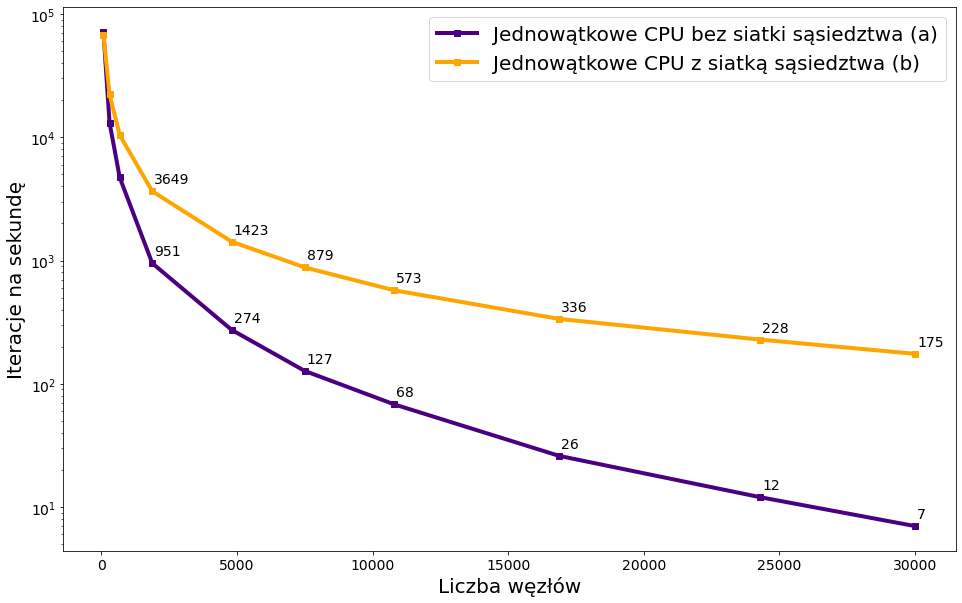
\includegraphics[width=18cm]{performance_cpu_grid_nogrid.png}
        \caption{
            Liczba iteracji na sekundę w zależności od ilości węzłów -
            węzły brzegowe i węzły brzegowe + siatka sąsiedztwa
        }
    \end{figure}
    Połączenie metody optymalizującej poprzez odrzucenie węzłów niebrzegowych wraz z umieszczeniem każdego węzła
    w siatce i branie pod uwagę jedynie węzły znajdującej się w tej samej lub w sąsiadującej komórce daje 
    bardzo dużą poprawę wydajności. Dla liczby węzłów $>15000$ wzrost iteracji na sekundę jest ponad 
    dziesięciokrotny na korzyść wersji algorytmu wykorzystującego obie metody optymalizacji.

    % --------------------------------------------------------------------------------------------------------------
    \subsection{Porównanie wydajności na CPU}
    \begin{figure}[H]
        \centering
        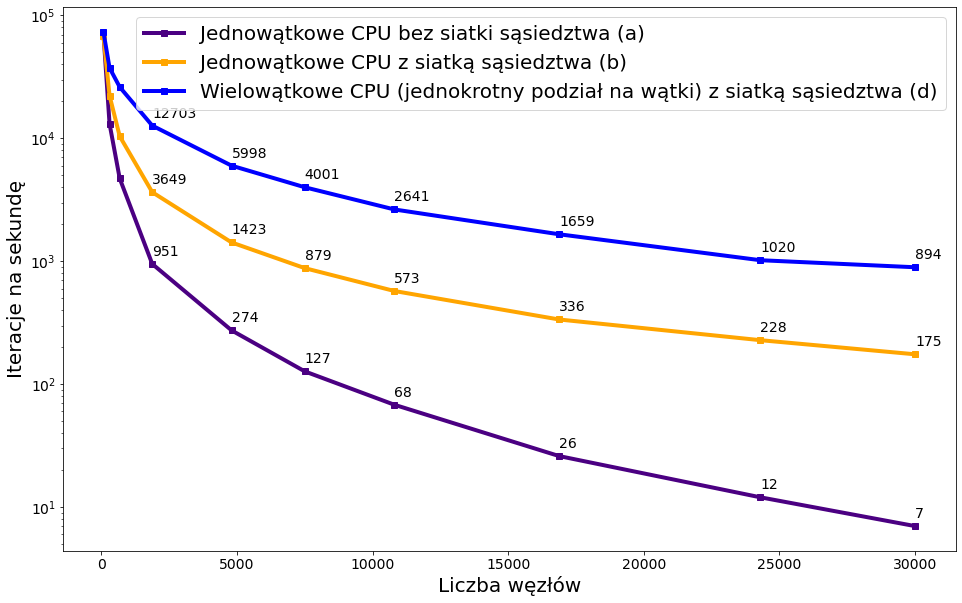
\includegraphics[width=18cm]{performance_cpu_best_worst.png}
        \caption{
            Liczba iteracji na sekundę w zależności od ilości węzłów
        }
    \end{figure}
    Następnym krokiem wykonanym w celu zwieszenia wydajności programu algorytmy zostały 
    zrównoleglone, dzięki czemu możemy zaobserwować następny skok wydajności. Procesor na którym 
    wykonywane były obliczenia posiada sześć rdzeni a uzyskane przyśpieszenie jest niemal pięciokrotne
    dla liczby węzłów $>20000$ co oznacza, że większość obliczeń udało się skutecznie zrównoleglić.

    % --------------------------------------------------------------------------------------------------------------
    \subsection{Porównanie wydajności wersji CPU i GPU}
    \begin{figure}[H]
        \centering
        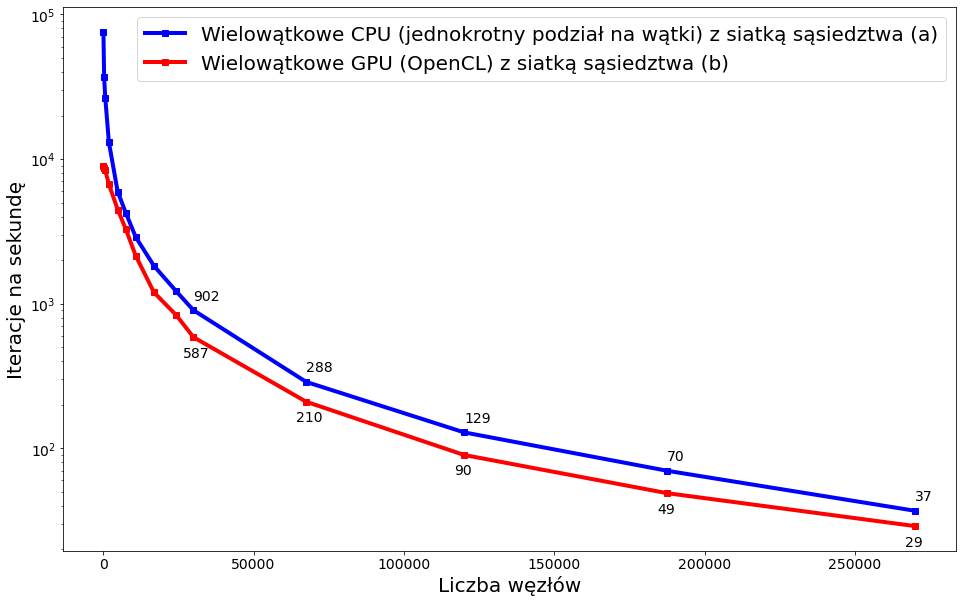
\includegraphics[width=18cm]{performance_best_cpu_gpu.png}
        \caption{
            Liczba iteracji na sekundę w zależności od ilości węzłów
        }
    \end{figure}
    Wersja wykonywana na CPU jest nieco szybsza niż ta wykonywana na GPU.
    Raportowane przez menażer zadań systemu Windows zużycie procesora graficznego podczas testu
    nie przekracza $30\%$ a zużycie CPU jest również niskie. Może to wynikać z 
    dużej ilości danych które muszą zostać skopiowane do pamięci karty graficznej, dlatego 
    duża część czasu obliczeniowego nie jest w pełni utylizowana.

    % --------------------------------------------------------------------------------------------------------------
    \subsection{Różnica pomiędzy najlepszą i najgorszą wydajnością}
    \begin{figure}[H]
        \centering
        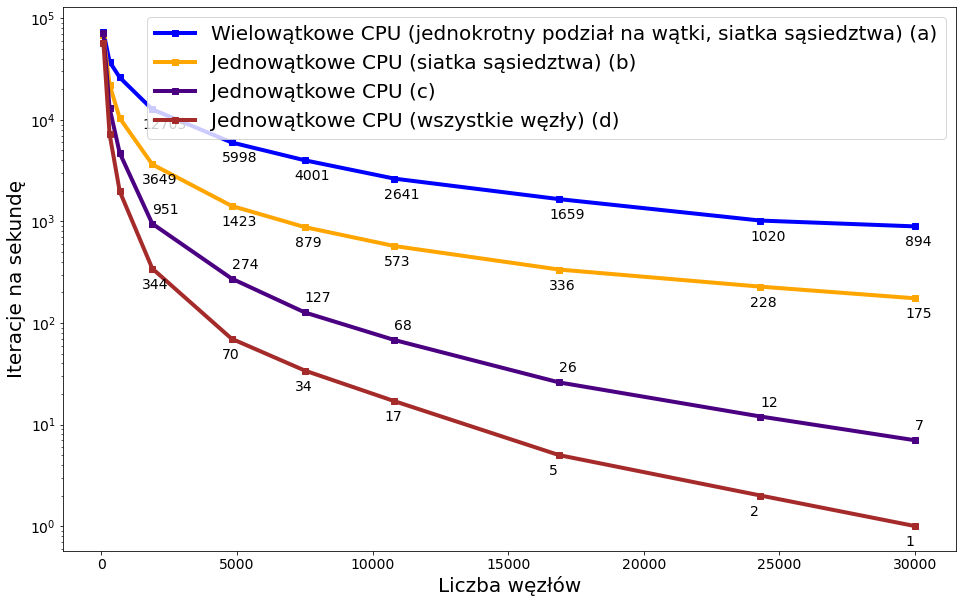
\includegraphics[width=16cm]{performance_all_best_worst.png}
        \caption{
            Liczba iteracji na sekundę w zależności od ilości węzłów -
            oś iteracji na sekundę przedstawiona jest w skali logarytmicznej
        }
    \end{figure}

    \begin{figure}[H]
        \centering
        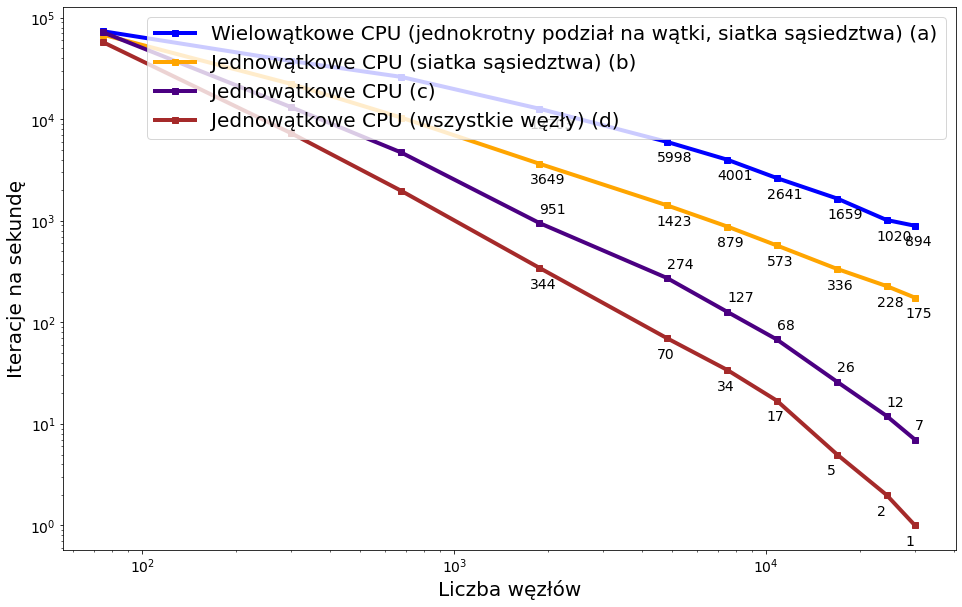
\includegraphics[width=16cm]{performance_all_best_worst_log_log.png}
        \caption{
            Liczba iteracji na sekundę w zależności od ilości węzłów - 
            obydwie osie przedstawione są w skali logarytmicznej
        }
    \end{figure}


    Po dokonaniu analizy zbiorczej wyników dla wszystkich wersji algorytmu możemy zauważyć, że
    ważniejszym aspektem podczas prób zwiększenia wydajności obliczeniowej algorytmów niż zrównoleglenie 
    jest optymalizacja wykonywanych obliczeń na przykład poprzez odrzucenie elementów nie wpływających 
    lub znikomo wpływających na wynik obliczeń. Aspekt ten można zauważyć na podstawie powyższego wykresu
    gdzie zmiany w algorytmie są w stanie przyśpieszyć działanie symulacji o ponad trzy rzędy wielkości w
    wybranych sytuacjach, podczas gdy samo zrównoleglenie wykonywania obliczeń jest ograniczone przez
    ilość dostępnych wątków obliczeniowych, przez co uzyskane w ten sposób przyśpieszenie działania 
    programu jest znacznie mniej efektowne. \\
    
    Oczywiście nie oznacza to, że nie warto zrównoleglić obliczeń
    jeżeli mamy taką możliwość, warto jednak pamiętać, że niezoptymalizowanych algorytm działający 
    na wielu rdzeniach obliczeniowych w większości przypadków będzie wyraźnie wolniejszy niż dobrze
    zoptymalizowany algorytm działający na jednym wątku obliczeniowym.

    \clearpage
    % --------------------------------------------------------------------------------------------------------------
    \section{Test rozrywania dwóch obiektów}
    \subsection{Opis testu}
    Scena składa się z dwóch nieruchomych obiektów, gdzie jeden o wymiarach $12 \times 24$ zostaje umieszczony nieruchomo 
    przy podłożu a drugi o wymiarach $2 \times 2$ znajduje się nad obiektem pierwszym. Siła grawitacji jest aktywna co 
    sprawia że obiekt drugi zaczyna spadać w kierunku obiektu pierwszego i po chwili następuje zderzenie. 
    Symulacja jest wykonywana dopóki układ nie znajduje się w stanie równowagi rozumianym jako wygaśnięcie ruchu
    węzłów.\\ 

    Jeżeli odległość między dwoma połączonymi węzłami zwiększy się powyżej $1.5$ odległości równowagi dla 
    tego połączenia ($d_x$), połączenie to zostaje zerwane - w ten sposób symulujemy rozrywanie obiektów pod dużym 
    obciążeniem. Do obsługi kolizji została użyta wersja algorytmu każdy węzeł z każdym węzłem, ponieważ
    działa on poprawnie dla przenikających się obiektów a przy relatywnie niewielkiej liczbie 
    węzłów ($4$ i $288$) wciąż zapewnia bardzo dobrą płynność działania animacji.


    \begin{multicols}{2}
        [
            \subsection{Parametry symulacji}
            Do symulacji zostały wykorzystane poniższe parametry:
        ]

        \begin{itemize}
            \item $g = 9.81$
            \item $dt = 10^{-5}$
        \end{itemize}
        Odpychanie międzyobiektowe (parametry potencjału Lennarda-Jonesa dla dwóch zderzających się obiektów):
        \begin{itemize}
            \item $V_{0} = 20$
            \item $d_{0} = 0.07$
        \end{itemize}
        Parametry obiektu $12 \times 24$:
        \begin{itemize}
            \item $c_{1} = 5.0$
            \item $m_{1} = 1.0$
            \item $d_{1} = 0.08$
            \item $V_{1} = 70.0$
            \item $r_{1} = [-0.92, -0.925]$
        \end{itemize}
        Parametry obiektu $2 \times 2$:
        \begin{itemize}
            \item $c_{2} = 1.0$
            \item $m_{2} = 30.0, 50.0, 80.0$
            \item $d_{2} = 0.15$
            \item $V_{2} = 500.0$
            \item $r_{2} = [-0.12, 0.8]$
        \end{itemize}
    \end{multicols}

    Parametry $r_x$ oznaczają pozycję początkową obiektu, $m_x$ masę węzłów w obiekcie, 
    $d_x$ pozycję równowagi przyciągania/odpychania pomiędzy dwoma węzłami dla tego
    samego obiektu lub jedynie odpychania dla oddziaływań międzywęzłowych,
    $V_x$ współczynnik oddziaływania międzywęzłowego, $g$ przyśpieszenie grawitacyjne, 
    $c_x$ współczynnik oporu dla każdego z węzłów w danym obiekcie.

    \clearpage
    \subsection{Wyniki}
    \subsubsection{Spadek obiektu o masie 120 kg w polu grawitacyjnym}
    \begin{figure}[h]

        \begin{subfigure}{0.5\textwidth}
            \centering
            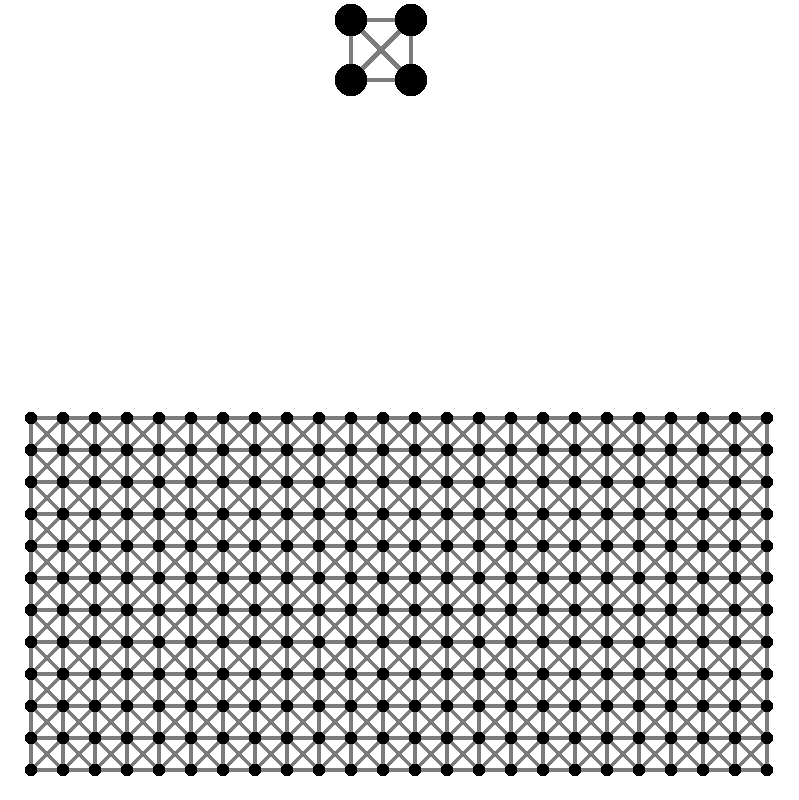
\includegraphics[width=6cm, height=6cm]{collision_2x2_24x12_mass30_1} 
            \caption{Stan początkowy}
        \end{subfigure}
        \begin{subfigure}{0.5\textwidth}
            \centering
            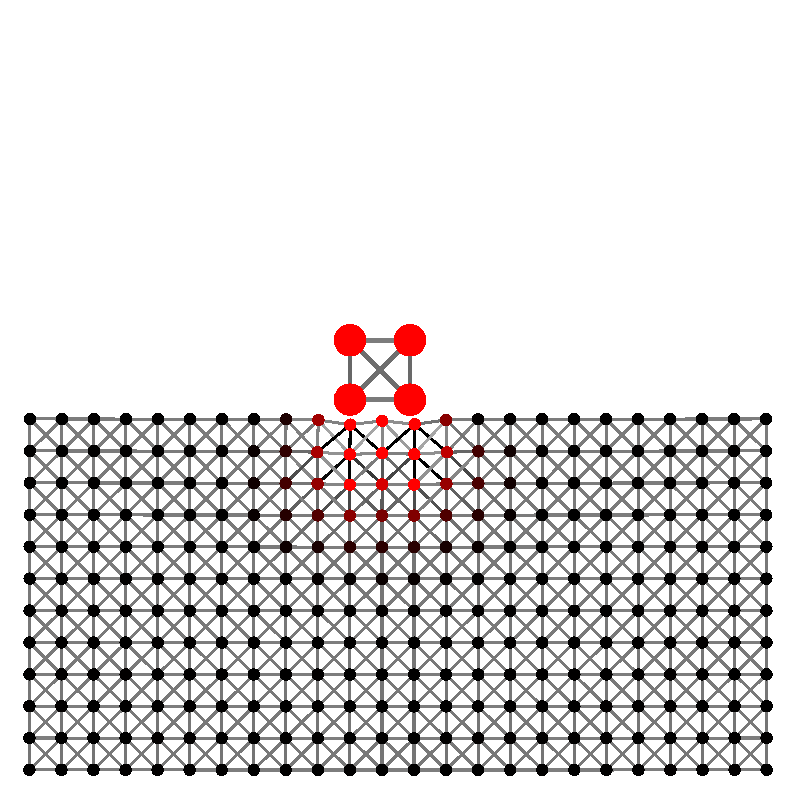
\includegraphics[width=6cm, height=6cm]{collision_2x2_24x12_mass30_2}
            \caption{Zderzenie}
        \end{subfigure}
        \begin{subfigure}{0.5\textwidth}
            \centering
            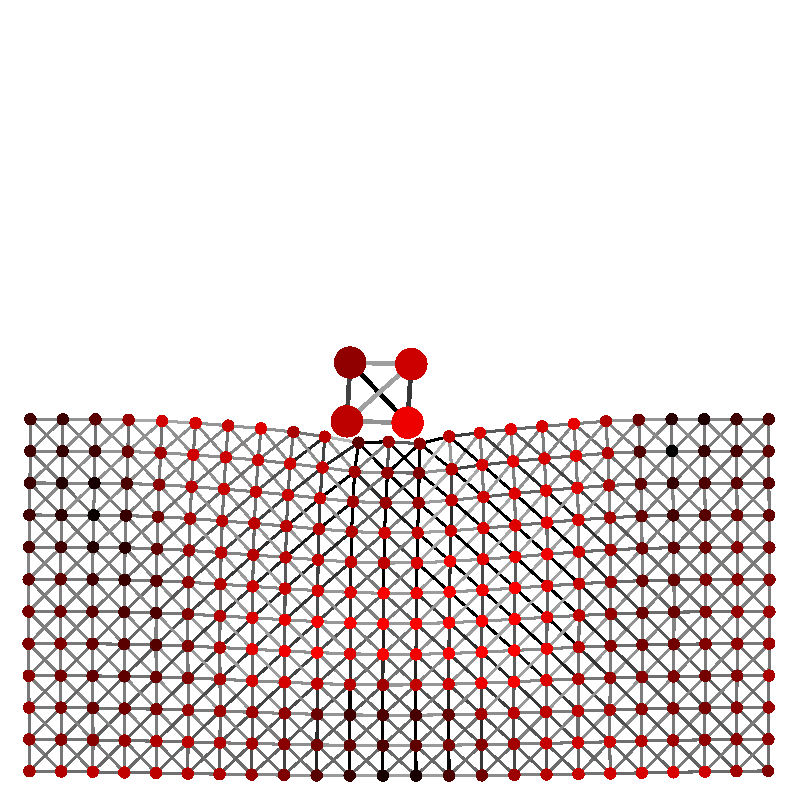
\includegraphics[width=6cm, height=6cm]{collision_2x2_24x12_mass30_3}
            \caption{Chwila po zderzeniu}
        \end{subfigure}
        \begin{subfigure}{0.5\textwidth}
            \centering
            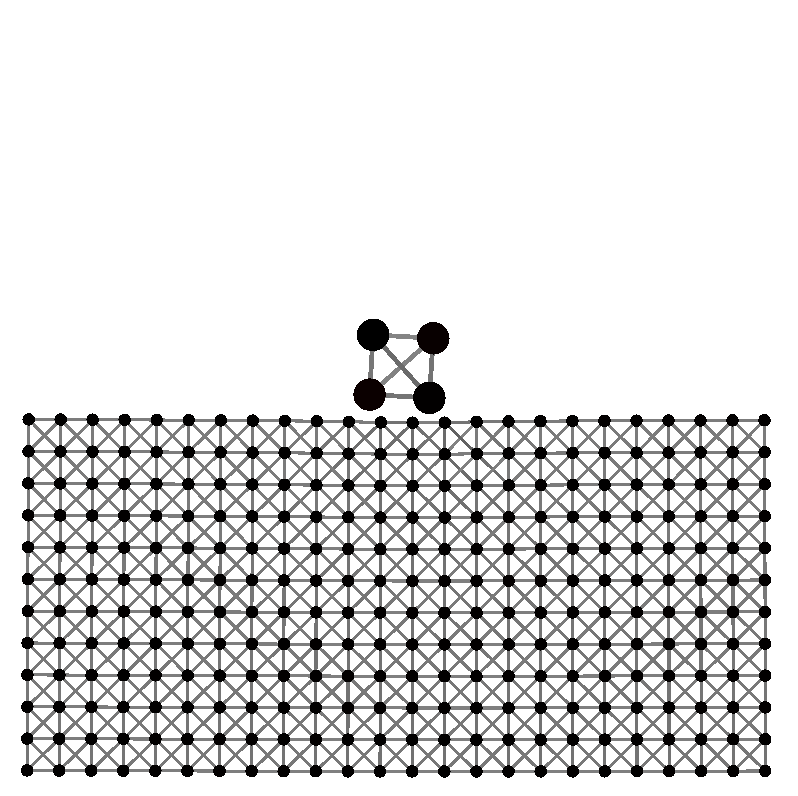
\includegraphics[width=6cm, height=6cm]{collision_2x2_24x12_mass30_4}
            \caption{Stan równowagi}
        \end{subfigure}
        
        \caption{Zderzenie spadającego obiektu $2 \times 2$ o masie 120 kg na obiekt $12 \times 24$ o masie 288 kg}
    \end{figure}
    Masa pojedynczego węzła w wolno spadającym obiekcie wynosi 30 kg co daje łączną masę równą 120 kg.
    Węzły o kolorze czarnym mają zerową energię kinetyczną, 
    zmieniają kolor na czerwony proporcjonalnie do ilości posiadanej energii kinetycznej. 
    Przy zderzeniu widoczny jest transfer energii kinetycznej z obiektu $2 \times 2$ do obiektu $12 \times 24$, 
    w którym po chwili zaczyna rozchodzić się fala. Ze względu na zastosowanie siły oporu proporcjonalnej do prędkości
    po kilku sekundach układ stabilizuje się, obiekt $2 \times 2$ leży nieruchomo na obiekcie $12 \times 24$. 
    Żadne z połączeń międzywęzłowych nie zostało przerwane ze względu na zbyt niską energię zderzenia.

    \clearpage
    \subsubsection{Spadek spadek obiektu o masie 200 kg w polu grawitacyjnym}
    \begin{figure}[h]

        \begin{subfigure}{0.5\textwidth}
            \centering
            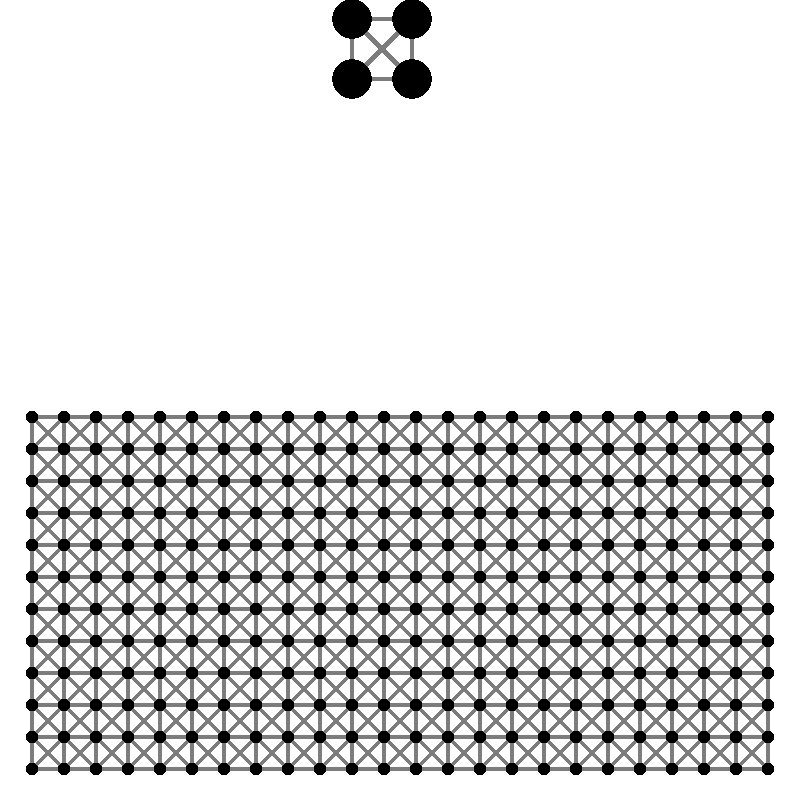
\includegraphics[width=6cm, height=6cm]{collision_2x2_24x12_mass50_1} 
            \caption{Stan początkowy}
        \end{subfigure}
        \begin{subfigure}{0.5\textwidth}
            \centering
            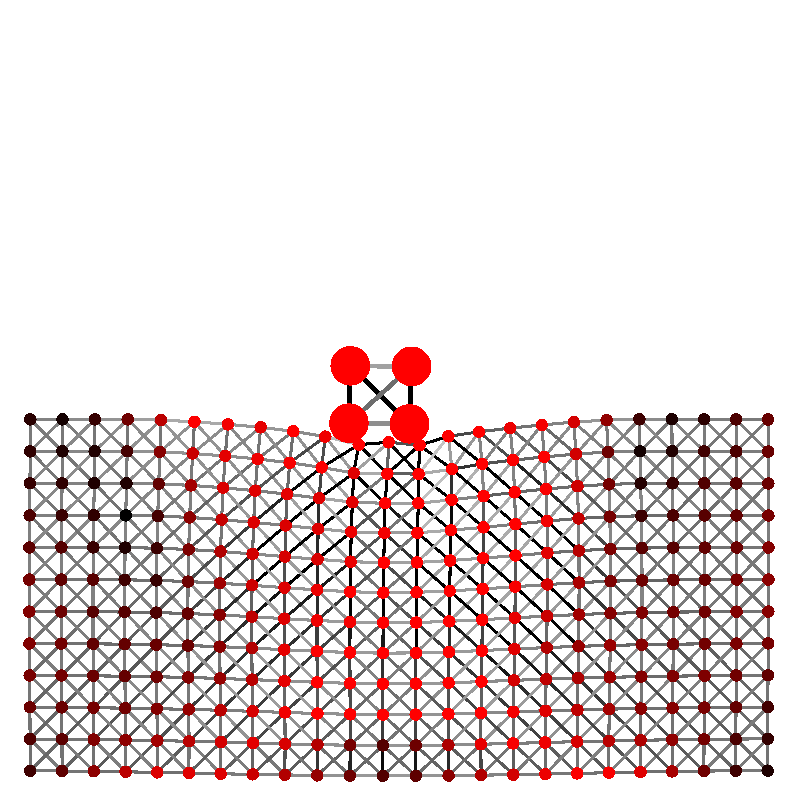
\includegraphics[width=6cm, height=6cm]{collision_2x2_24x12_mass50_2}
            \caption{Zderzenie}
        \end{subfigure}
        \begin{subfigure}{0.5\textwidth}
            \centering
            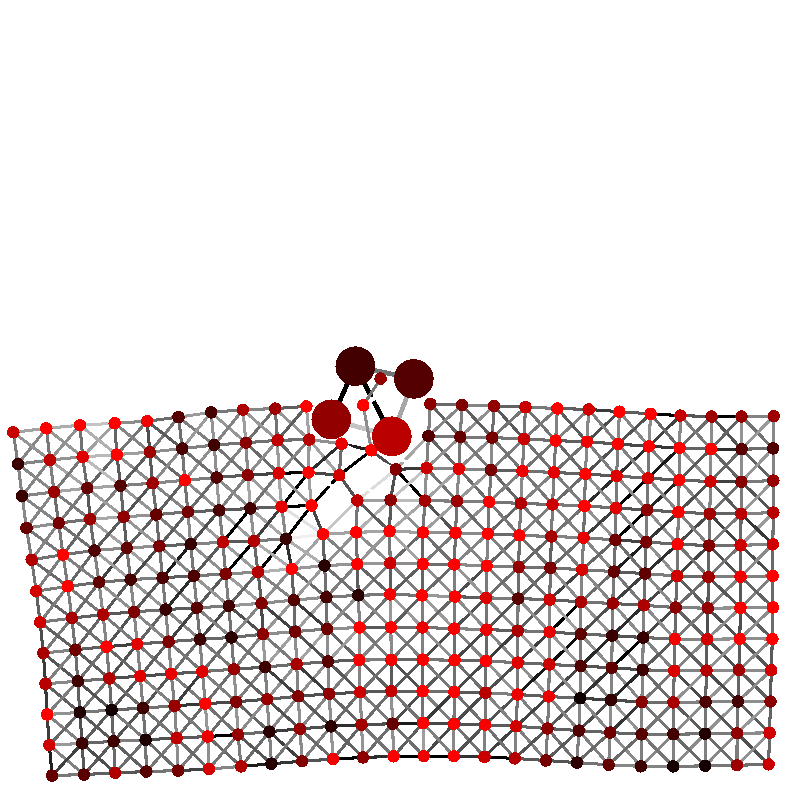
\includegraphics[width=6cm, height=6cm]{collision_2x2_24x12_mass50_3}
            \caption{Chwila po zderzeniu}
        \end{subfigure}
        \begin{subfigure}{0.5\textwidth}
            \centering
            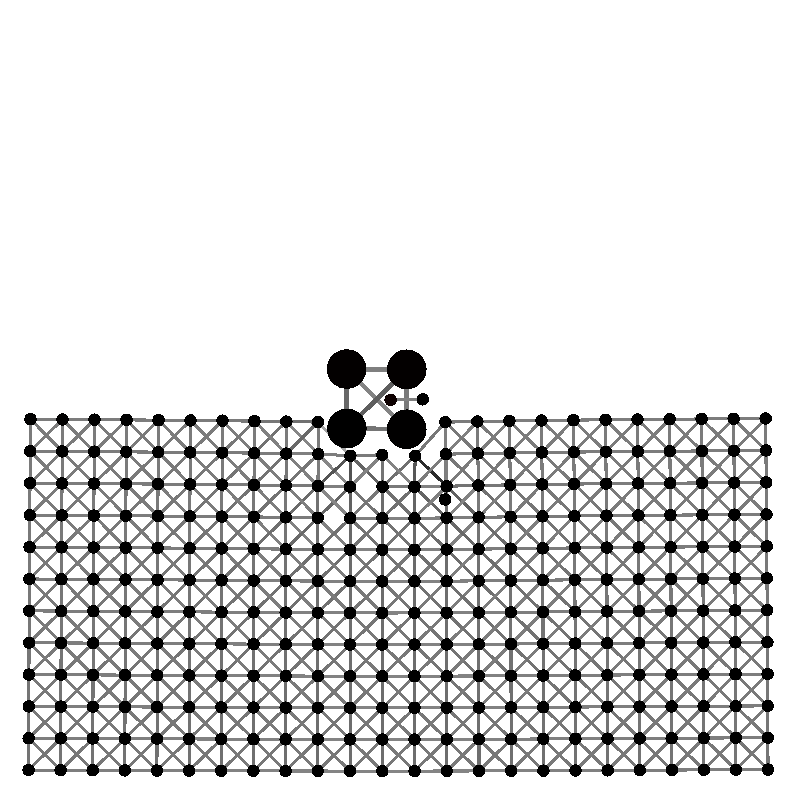
\includegraphics[width=6cm, height=6cm]{collision_2x2_24x12_mass50_4}
            \caption{Stan równowagi}
        \end{subfigure}
        
        \caption{Zderzenie spadającego obiektu $2 \times 2$ o masie 200 kg na obiekt $12 \times 24$ o masie 288 kg}
    \end{figure}

    Zwiększamy masę węzłów w obiekcie $2 \times 2$ z 30 kg do 50 kg. Ponieważ w reprezentacja wizualnej węzła jego pole 
    jest proporcjonalne do jego masy, tym razem obiekt $2 \times 2$ jest większy.
    Większa energia kinetyczna przy zderzeniu powoduje przerwanie kilku połączeń międzywęzłowych, a obiekt $2 \times 2$ 
    utyka w wytworzonej wnęce. Część pierwotnego obiektu $12 \times 24$ oderwała się i utknęła w obiekcie $2 \times 2$.

    \clearpage
    \subsubsection{Spadek spadek obiektu o masie 320 kg w polu grawitacyjnym}
    \begin{figure}[h]

        \begin{subfigure}{0.5\textwidth}
            \centering
            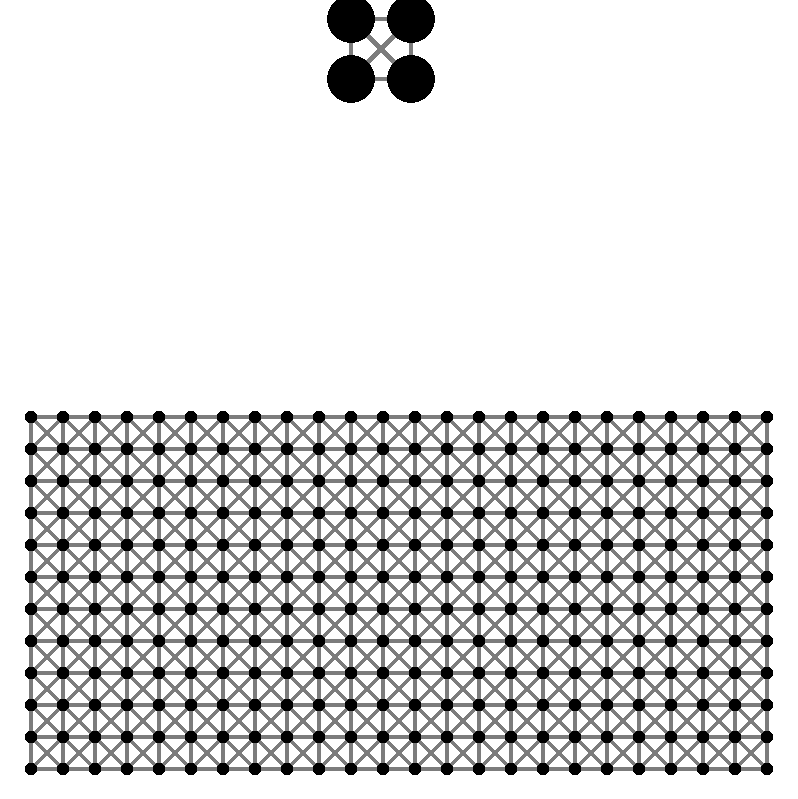
\includegraphics[width=6cm, height=6cm]{collision_2x2_24x12_mass80_1} 
            \caption{Stan początkowy}
        \end{subfigure}
        \begin{subfigure}{0.5\textwidth}
            \centering
            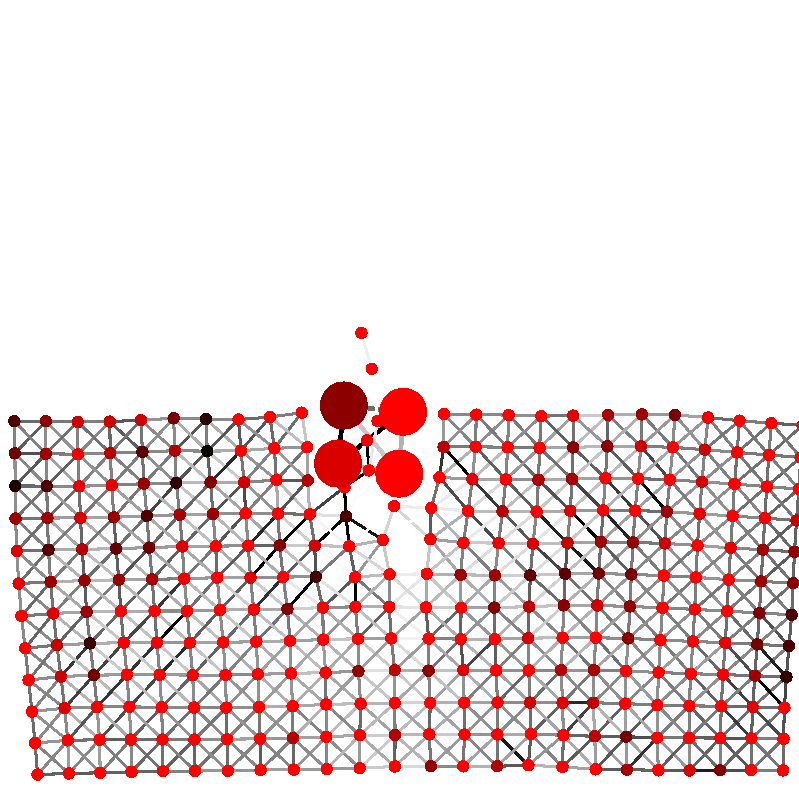
\includegraphics[width=6cm, height=6cm]{collision_2x2_24x12_mass80_2}
            \caption{Zderzenie}
        \end{subfigure}
        \begin{subfigure}{0.5\textwidth}
            \centering
            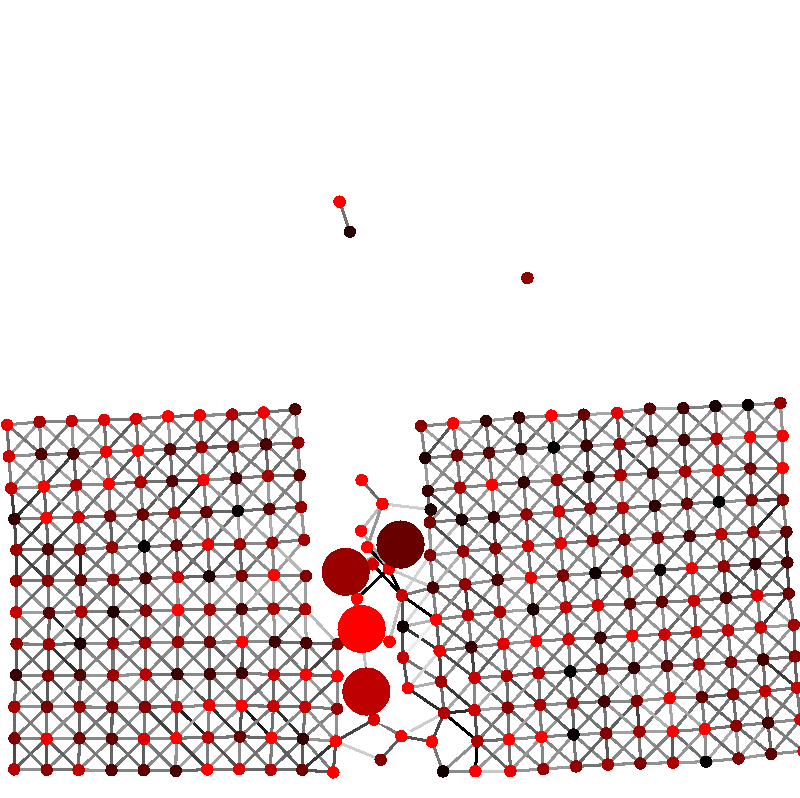
\includegraphics[width=6cm, height=6cm]{collision_2x2_24x12_mass80_3}
            \caption{Chwila po zderzeniu}
        \end{subfigure}
        \begin{subfigure}{0.5\textwidth}
            \centering
            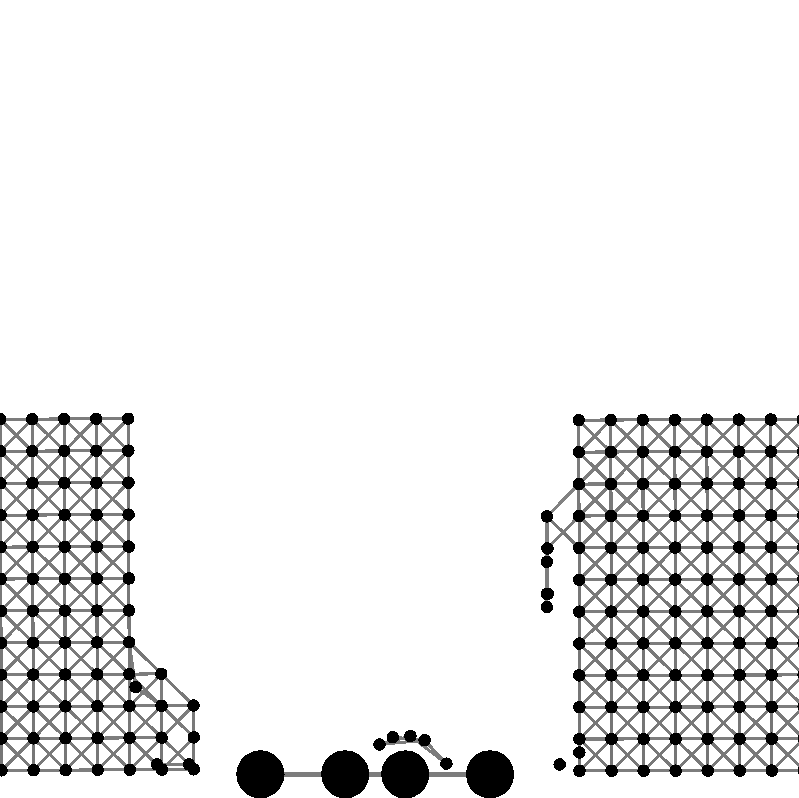
\includegraphics[width=6cm, height=6cm]{collision_2x2_24x12_mass80_4}
            \caption{Stan równowagi}
        \end{subfigure}
        
        \caption{Zderzenie spadającego obiektu $2 \times 2$ o masie 320 kg na obiekt $12 \times 24$ o masie 288 kg}
    \end{figure}

    Ponowne zwiększona została masa węzłów obiektu $2 \times 2$, tym razem z 50 kg do 80 kg, dając łączną masę 320 kg.
    W chwili zderzenia po obiekcie $12 \times 24$ rozchodzi się gwałtownie fala energii kinetycznej a on sam zostaje 
    rozerwany. Częściowemu zniszczeniu ulega również obiekt $2 \times 2$, ze względu duży stosunek masy do wytrzymałości
    połączeń międzywęzłowych niektóre z tych połączeń zostały przerwane.

    % --------------------------------------------------------------------------------------------------------------
    \clearpage
    \section{Test widoku ciśnienia dla jednego obiektu}
    \subsection{Opis testu}
    Jeden obiekt o wymiarach $50 \times 50$ węzłów umieszczony zostaje przy podłożu w polu grawitacyjnym.
    Konsystencja obiektu przypomina galaretę, nie jest on sztywny. W czasie trwania symulacji 
    aktywna jest siła oporu o wysokiej wartości proporcjonalna do prędkości węzła, co powoduję szybką 
    utratę energii.

    \subsection{Reprezentacja graficzna w czasie}

    \begin{figure}[h]

        \begin{subfigure}{0.5\textwidth}
            \centering
            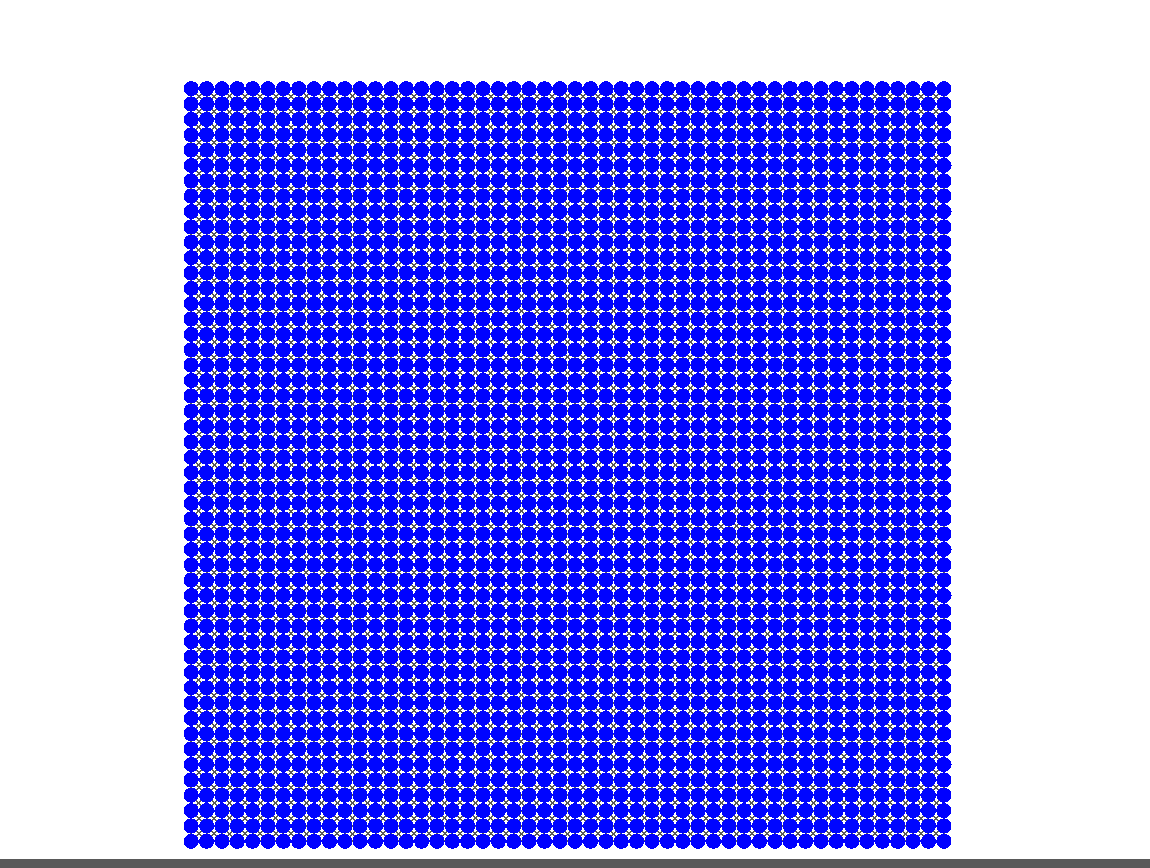
\includegraphics[width=6cm, height=4.5cm]{pressure_01.png} 
            \caption{Stan początkowy}
        \end{subfigure}
        \begin{subfigure}{0.5\textwidth}
            \centering
            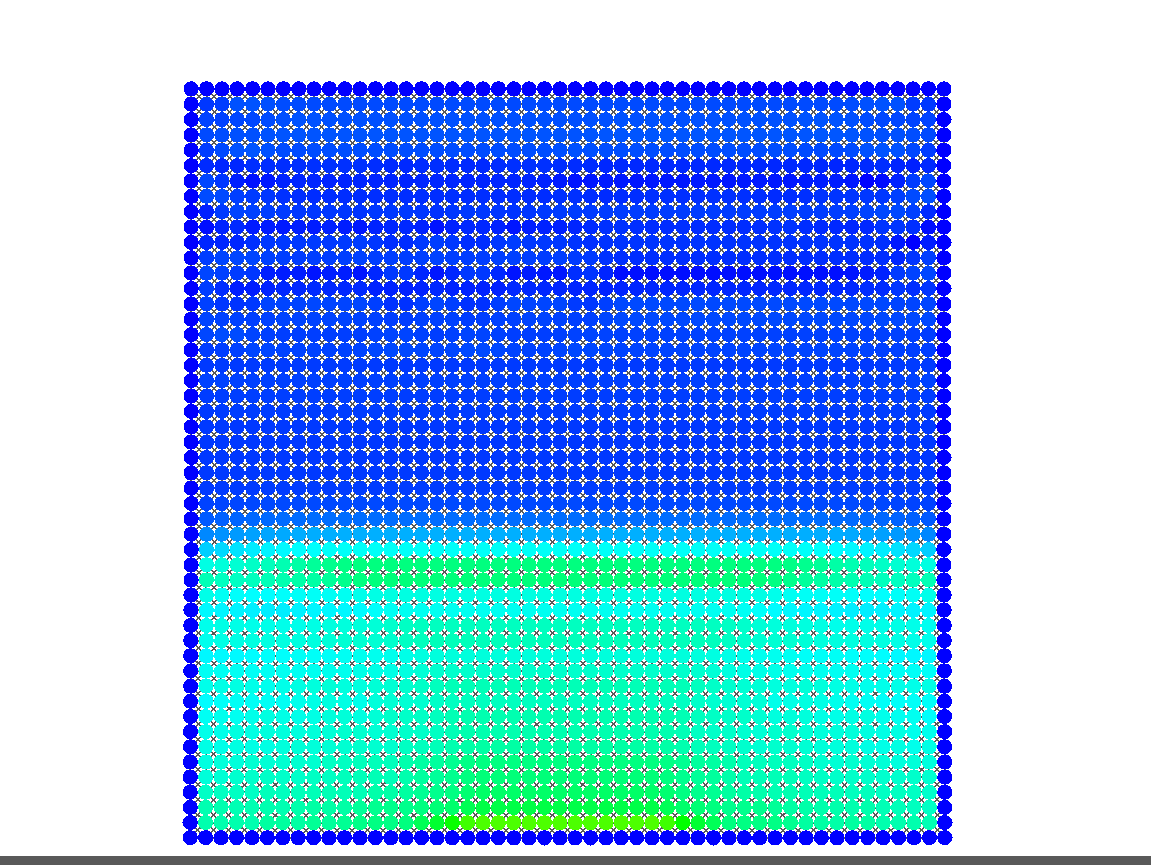
\includegraphics[width=6cm, height=4.5cm]{pressure_02.png}
            \caption{Propagacja fali ciśnienia}
        \end{subfigure}
        \begin{subfigure}{0.5\textwidth}
            \centering
            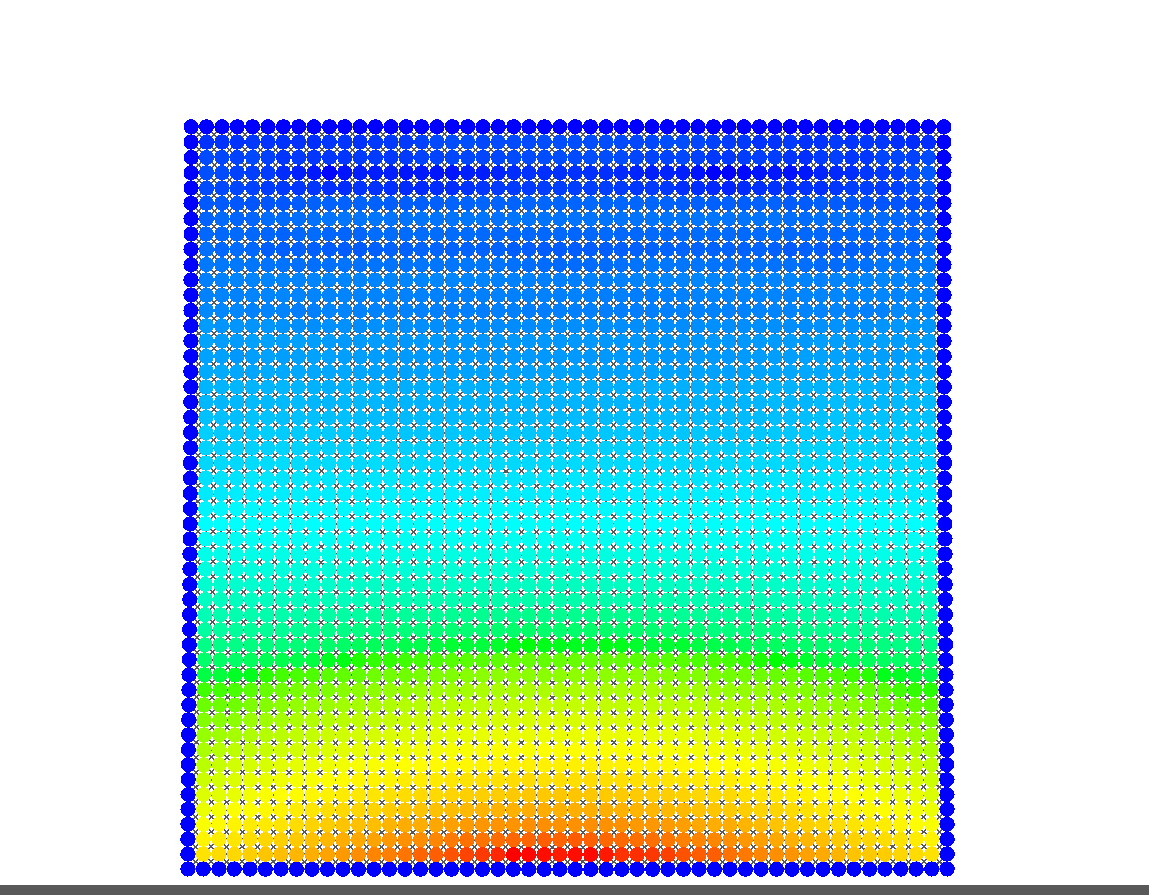
\includegraphics[width=6cm, height=4.5cm]{pressure_03.png}
            \caption{Stabilizacja rozkładu ciśnienia}
        \end{subfigure}
        \begin{subfigure}{0.5\textwidth}
            \centering
            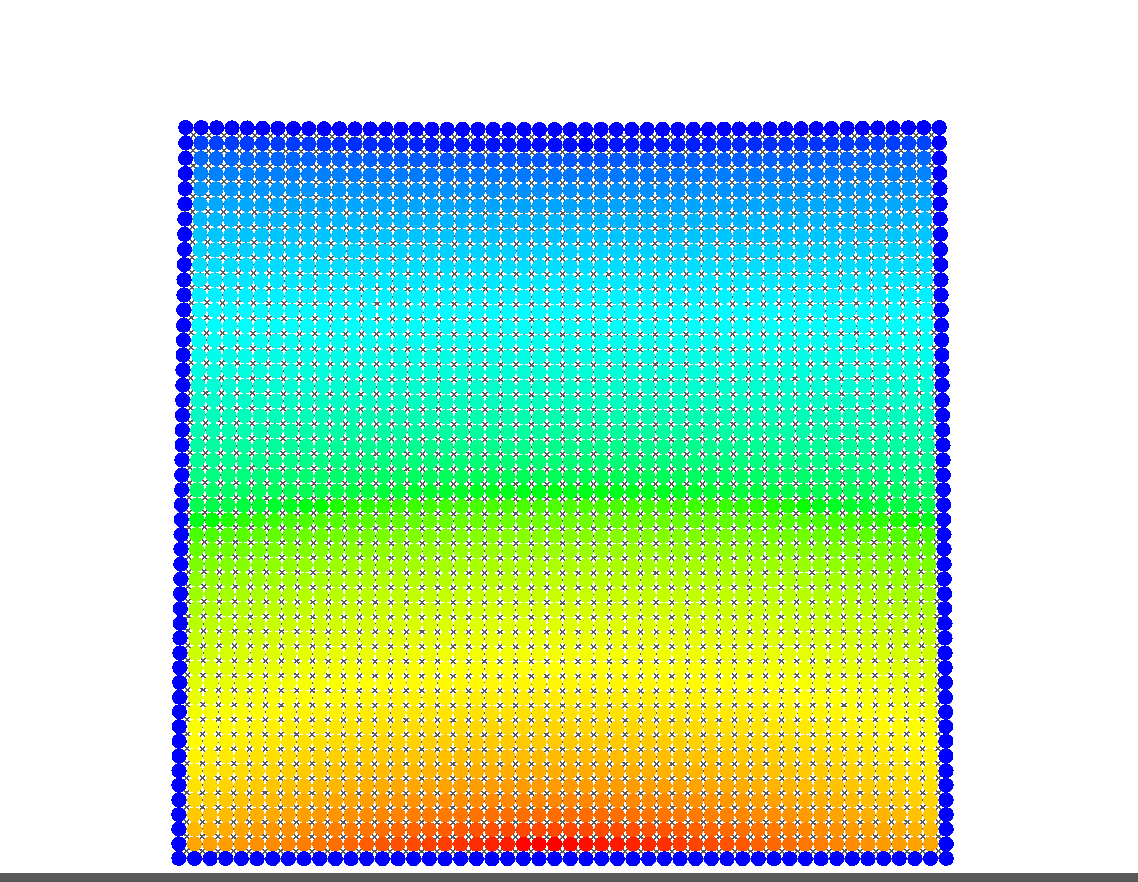
\includegraphics[width=6cm, height=4.5cm]{pressure_04.png}
            \caption{Stan równowagi}
        \end{subfigure}
        
        \caption{Widok ciśnienia w wybranych chwilach czasowych dla obiektu $50 \times 50$}
    \end{figure}

    Węzły na które oddziałuje najmniejsze ciśnieniu mają kolor ciemno-niebieski, natomiast węzły na które oddziałuje 
    największe ciśnienie mają kolor czerwony. Ponieważ podczas obliczania ciśnienia bierzemy pod uwagę jedynie 
    siły oddziaływania pomiędzy połączonymi sąsiadami a węzły brzegowe mają mniej sąsiadów niż węzły znajdujące
    się w środku obiektu, to ciśnienie działające na węzły zewnętrzne będzie mniejsze niż to działające na
    węzły wewnętrzne, z czego wynika widoczne ciemno-niebieskie obramowanie obiektu. \\

    Na początku symulacji można zauważyć przemieszczającą się w górę obiektu falę ciśnienia. Wraz z czasem 
    obiekt stał się również bardziej wypukły od strony prawej i lewej ścianki
    oraz wklęsły od strony górnej ścianki. W stanie stabilnym jest on również niższy niż na początku symulacji 
    Największe ciśnienie można zaobserwować przy środku podstawy obiektu a najmniejsze przy jego 
    górnej ściance.

    \subsection{Zmiana energii układu w czasie}
    Pomiar energii pozwala na głębsze zrozumienie zmian zachodzących w układu podczas
    wykonywania testu.

    \begin{figure}[H]
        \centering
        \includegraphics[width=14cm]{pressure_energy_01}
        \caption{
            Zmiana energi układu w czasie dla pierwszych 0.5 sekundy
        }
    \end{figure}

    Widoczna jest utrata energii całkowitej reprezentowanej przez linię o kolorze czarnym, która po około $0.3$ sekundy
    stabilizuje się. Energia potencjalna grawitacji również spada, co odpowiada wcześniej zaobserwowanej 
    zmniejszającej się wraz z czasem wysokości obiektu.

    \begin{figure}[H]
        \centering
        \includegraphics[width=14cm]{pressure_energy_02.png}
        \caption{
            Zmiana energi układu w czasie dla pierwszych 3.0 sekundy
        }
    \end{figure}

    Gasnące oscylacje energi potencjalnej grawitacji oraz energi potencjalnej Lennarda-Jonesa wewnątrz obiektu
    wynika z niewielkich drgań w które wpadł obiekt. Jego konsystencja przypomina galaretę, więc spodziewalibyśmy się
    oscylacji energii tego typu, jednak ze względu na istnienie siły oporu po kilku sekundach drgania te wygaszają się.

    % --------------------------------------------------------------------------------------------------------------
    \subsection{Największa wartość ciśnienia na węźle w czasie}
    Pozwala lepiej zrozumieć kolory.

    \begin{figure}[H]
        \centering
        \includegraphics[width=14cm]{pressure_pressure_01}
        \caption{
            Największa wartość ciśnienia na węźle w czasie dla pierwszych 0.5 sekundy
        }
    \end{figure}

    Szybki wzrost.

    \begin{figure}[H]
        \centering
        \includegraphics[width=14cm]{pressure_pressure_02}
        \caption{
            Największa wartość ciśnienia na węźle w czasie dla pierwszych 3.0 sekundy
        }
    \end{figure}

    Oscylacje.


    \clearpage
    % --------------------------------------------------------------------------------------------------------------
    \section{Rozkład ciśnienia podczas zderzenia dwóch obiektów}
    \subsection{Opis testu}
    Jeden obiekt o wymiarach $50 \times 50$ węzłów umieszczony zostaje przy podłożu w polu grawitacyjnym a
    drugi obiekt o wymiarach $20 \times 20$ znajduje się nad obiektem pierwszym. Po krótkimi czasie pod wpływem
    działania siły grawitacji obiekt drugi zderza się z obiektem pierwszym. Aktywna jest siła oporu 
    proporcjonalna do prędkości węzła, co powoduje straty energii całkowitej układu i po pewnym czasie osiągnięcie
    stanu równowagi.

    \subsection{Reprezentacja graficzna w czasie}

    \begin{figure}[h]

        \begin{subfigure}{0.5\textwidth}
            \centering
            \includegraphics[width=6cm, height=5.5cm]{pressure02_01} 
            \caption{Stan początkowy}
        \end{subfigure}
        \begin{subfigure}{0.5\textwidth}
            \centering
            \includegraphics[width=6cm, height=5.5cm]{pressure02_02}
            \caption{Przed zderzeniem}
        \end{subfigure}
        \begin{subfigure}{0.5\textwidth}
            \centering
            \includegraphics[width=6cm, height=5.5cm]{pressure02_03}
            \caption{Zderzenie}
        \end{subfigure}
        \begin{subfigure}{0.5\textwidth}
            \centering
            \includegraphics[width=6cm, height=5.5cm]{pressure02_04}
            \caption{Stan równowagi}
        \end{subfigure}
        
        \caption{Widok ciśnienia w wybranych chwilach czasowych dla zderzenia obiektów $50 \times 50$ i $20 \times 20$}
    \end{figure}

    Przed zderzeniem największe ciśnienie w obiekcie pierwszym znajduje się na węzłach przy jego podstawie 
    a w obiekcie drugim nie występują żadne różnice ciśnień. Stan ten zmienia się w momencie zderzenia, 
    gdzie największe ciśnienie można zaobserwować w miejscu kontaktu obiektów. W stanie stabilnym 
    można zauważyć, że ze względu na niesymetryczne rozłożenie węzłów, ciśnienie przy podstawie 
    obiektu $50 \times 50$ jest wyraźnie wyższe po jego lewej stronie w porównaniu do strony prawej. \\

    Warto zwrócić uwagę że dany kolor nie jest jest bezpośrednio odwzorowywany na jedną wartość przez cały
    czas trwania symulacji. Kolorem czerwonym zawsze oznaczony jest węzeł o największej wartości a 
    kolorem ciemno-niebieskim węzeł o najmniejszej wartości. Z tego powodu na rysunku
    przedstawiającym moment zderzenia kolor węzłów przy podstawie obiektu $50 \times 50$ zmienił się z 
    czerwonego na żółty, pomimo iż wartość ciśnienia w tamtym miejscu wzrosła. Kolorem 
    czerwonym oznaczone zostały w tej chwili czasowej węzły w miejscu kontaktu obiektów, gdzie wartość 
    ciśnienia była większa niż przy podstawie obiektu $50 \times 50$.

    \subsection{Zmiana energii układu w czasie}
    \begin{figure}[H]
        \centering
        \includegraphics[width=16cm]{pressure_energy02_01}
        \caption{
            Zmiana energi układu w czasie dla pierwszych 0.35 sekundy
        }
    \end{figure}
    
    Energia potencjalna grawitacji zmniejsza się głównie ze względu na spadający obiekt $20 \times 20$
    a ponieważ utrata energii układu jest proporcjonalna do prędkości węzłów, na początku symulacji gdy 
    obiekty są nieruchome i dopiero nabierają prędkości energia całkowita zmniejsza się w wolniejszym tempie niż 
    w późniejszym etapie symulacji, gdy węzły mają już znaczącą prędkość.

    \begin{figure}[H]
        \centering
        \includegraphics[width=16cm]{pressure_energy02_02}
        \caption{
            Zmiana energi układu w czasie dla pierwszych 1.6 sekundy
        }
    \end{figure}

    Ponieważ w tym przypadku następuje zderzenie pomiędzy obiektami energia potencjalna Lennarda-Jonesa odpychająca
    oznaczona linią o kolorze czerwonym nie jest stała i wzrasta w momencie zderzenia. W stanie spoczynku jej wartość
    jest większa niż na początku symulacji, ponieważ w stanie stabilnym obiekt $20 \times 20$ leży nieruchomo na obiekcie
    $50 \times 50$, a więc siła odpychająca między obiektami przeciwdziała sile grawitacji. 
    Wzrasta też oznaczona kolorem pomarańczowym energia odpychająca węzły od podłoża, gdyż po momencie zderzenia na 
    tym podłożu spoczywa również niebezpośrednio masa  obiektu $20 \times 20$. \\
    
    Zaobserwować można również wzrost oznaczonej linią zieloną energii międzywęzłowej wewnętrznej obiektu, wynikającej ze 
    zmniejszenia odległości pomiędzy węzłami na wskutek zgniecenia obiektu. Energia wewnętrzna wzrasta w dwóch momentach: 
    najpierw obiekt $50 \times 50$ zmienia swój kształt pod wpływem działania siły grawitacji, co powoduje zmniejszenie 
    odległości pomiędzy węzłami znajdującymi sę w nim, ten etap widoczny jest w przedziale czasu $[0, 0.6] s$. 
    Następnie w momencie $\approx 0.6 s$ następuje zderzenie powodujące wyraźne zgniecenie obiektu a zatem znaczny wzrost
    energii wewnętrznej międzywęzłowej. Energia ta po momencie zderzenia zmniejsza się na wskutek częściowego rozprężenia
    obiektów, jednak nie powraca do swojej poprzedniej wartości, ponieważ spoczywające na sobie obiekty nadal są 
    częściowo zniekształcone.

    % --------------------------------------------------------------------------------------------------------------
    \subsection{Największa wartość ciśnienia na węźle w czasie}
    Pozwala lepiej zrozumieć kolory.

    \begin{figure}[H]
        \centering
        \includegraphics[width=14cm]{pressure_pressure02_01}
        \caption{
            Największa wartość ciśnienia na węźle w czasie dla pierwszych 0.35 sekundy
        }
    \end{figure}

    Szybki wzrost.

    \begin{figure}[H]
        \centering
        \includegraphics[width=14cm]{pressure_pressure02_02}
        \caption{
            Największa wartość ciśnienia na węźle w czasie dla pierwszych 1.6 sekundy
        }
    \end{figure}

    Oscylacje.

\chapter{Podsumowanie}
    Zastosowanie metoda dynamiki molekularnej daje bardzo interesujące 
    wyniki podczas symulacji zderzeń obiektów. Zastosowanie dużej ilości węzłów pozwala na 
    ukazanie realistycznie wyglądających obiektów elastycznych zdolnych do kolizji między sobą 
    i rozrywających się gdy działa na nie odpowiednio duża siła. \\
    
    Konieczność wykonywania i wyświetlania symulacji z dużą ilością węzłów w czasie 
    rzeczywistym tworzy wiele problemów z wydajnością programu, wymagając
    od programisty kreatywnego podejścia do optymalizacji. Ukazuje również korzyści wynikające z 
    zastosowania zrównoleglenia algorytmów, pozwalając na wykonywanie ich znacznie znacznie szybciej na 
    urządzeniach wielowątkowych takich jak procesory czy karty graficzne. \\

    Gdy tworzymy algorytm mający działać na procesorze graficznym, bardzo istotnym aspektem jest 
    koszt związany z przesyłem danych z pamięci głównej do pamięci karty graficznej. Sam proces kopiowania 
    danych może poważnie wpłynąć na wydajność programu i w niektórych przypadkach może on zająć więcej
    czasu niż samo wykonanie obliczeń.
    ``Computing has (...) moved from one limited by computational throughput of the 
    processor, to one where moving the data is the primary limiting factor'' - \cite{cuda}. \\

    Podstawowym problemem jest wydajność, najpierw każdy węzeł był rysowany osobno ale to podejście 
    było zbyt wolne. Następnie przy użyciu renderowania instancyjnego (instanced rendering) 
    problem ten został zlikwidowany po stronie interfejsu graficznego. 
    Wydajność symulacji, jest dużym problem gdy ilość obiektów jest znacząca. 
    Zrównoleglenie algorytmów jest trudne do osiągnięcia, wymaga znacznej modyfikacji programu oraz często 
    wymaga pewnych ustępstw w celu zniwelowania niezdefiniowanego zachowania wynikającego z wyścigów 
    (\emph{race conditions}) dostępu do pamięci.

    % --------------------------------------------------------------------------------------------------------------
    % \section{Dodatek}
    % \subsection{Animacje prezentujące działanie aplikacji}
    
    % \subsubsection{Przekazanie energii między dwoma sztywnimi obiektami}
    % \url{https://youtu.be/nolLh6CSa-8} \\

    % Mniejszy obiekt $3 \times 3$ po odbiciu od większego obiektu $8 \times  8$ 
    % znajdującego się  pod nim wznosi się na
    % wysokość o wiele większą, niż ta z której rozpoczął spadek swobodny.
    % Występuje tutaj przekazanie części energii z obiektu 
    % większego do mniejszego - sama zasada energii jest zachowana.

    % \subsubsection{Przekazanie energii między dwoma miękkimi obiektami}
    % \url{https://youtu.be/q2uYx8uLl3w} \\

    % W tym przypadku obiekty są mniej sztywne, obiekt $3 \times 3$ po odbiciu 
    % od obiektu $8 \times  8$ wznosi się na wyraźnie mniejszą wysokość niż w przypadku bardziej sztywnych obiektów
    % (jednak wciąż wyżej niż punkt z którego zaczął spadać). Można to wytłumaczyć tym,
    % że znaczna część energii która w poprzednim przypadku była częścią ruchu postępowego,
    % teraz stała się energią wewnętrzną obiektów (wibracje obiektów pochłaniają część energii).

    % \subsubsection{Proste zderzenie dwóch obiektów}
    % \url{https://www.youtube.com/watch?v=4cGcL_5yUt4} \\ 

    % Przypadek pokazujący zderzenie dwóch obiektów nieznajdujących się w polu grawitacyjnym.
    % Jednemu z obiektów nadana jest prędkość początkowa, po chwili obiekty zderzają się i 
    % odbijają się od siebie.

    % \subsubsection{Zderzenie obiektów 120 kg z 288 kg}
    % \url{https://youtu.be/3dV6EpRacyA} \\

    % Wolny spadek, brak zniszczeń obiektów.

    % \subsubsection{Zderzenie obiektów 200 kg z 288 kg}
    % \url{https://youtu.be/lRGl7CJiqFU} \\

    % Wolny spadek, częściowe uszkodzenie jednego z obiektów.

    % \subsubsection{Zderzenie obiektów 320 kg z 288 kg}
    % \url{https://youtu.be/VYeCsaqNxAY} \\

    % Wolny spadek, pełne zniszczenie obydwóch obiektów.

    % \subsection{Repozytorium}
    % \subsubsection{Link do repozytorium z kodem}
    % \url{https://github.com/theYiome/elastic-objects-rs}

    \begin{thebibliography}{9}

        \bibitem{grafika3d}
        Jacek Matulewski (2014) 
        \emph{Grafika 3D czasu rzeczywistego. Nowoczesny OpenGL},
        Wydawnictwo Naukowe PWN SA, Wydanie I

        \bibitem{cuda}
        Shane Cook (2013) 
        \emph{CUDA Programming, a developer's guide to parallel computing with GPUs},
        Elsevier Inc., Morgan Kaufmann

        \bibitem{cleancode}
        Robert C. Martin (2014) 
        \emph{Czysty Kod, podręcznik dobrego programisty},
        Helion S.A.

        \bibitem{velocityverlet}
        Swope, William C.; H. C. Andersen; P. H. Berens; K. R. Wilson (1982) 
        \emph{A computer simulation method for the calculation of 
            equilibrium constants for the formation of physical clusters 
            of molecules: Application to small water clusters}, 
        The Journal of Chemical Physics. 76, 637 (Appendix)

        \bibitem{numerical}
        Tomasz Dziubak, Jacek Matulewski, Radosław Płoszajczak, Marcin Sylwestrzak (2014)
        \emph{Grafika Fizyka Metody Numeryczne - Symulacje fizyczne z wizualizacją 3D},
        Wydawnictwo Naukowe PWN SA

        \bibitem{moleculardynamics}
        M. Greibel, S. Knapek, G. Zumbusch (2007)
        \emph{
            Numerical Simulation in Molecular Dynamics – 
            numerics, algorithms, parallelization, applications},
        SPRINGER

        \bibitem{rustbook}
        Steve Klabnik, Carol Nichols (2022)
        \emph{The Rust Programming Language} \\
        \url{https://doc.rust-lang.org/book}

        \bibitem{rayon}
        Dokumentacja online biblioteki \emph{rayon 1.5.1} \\
        \url{https://docs.rs/rayon/1.5.1/rayon/}

        \bibitem{glium}
        Dokumentacja online biblioteki \emph{glium 0.30.2} \\
        \url{https://docs.rs/glium/0.30.2/glium/}

        \bibitem{egui}
        Dokumentacja online biblioteki \emph{egui 0.15.0} \\
        \url{https://docs.rs/egui/0.15.0/egui/}

    \end{thebibliography}

\end{document}